%
%   Prof. Dr. Julian Reichwald  
%   auf Basis einer Vorlage von Prof. Dr. Jörg Baumgart
%   DHBW Mannheim 
%  
%
%	ACHTUNG: Für das Erstellen des Literaturverzeichnisses wird das modernere Paket biblatex
%			 in Kombination mit biber verwendet -- nicht mehr das ältere BibTex!  
% 			 Bitte stellen Sie ggf. Ihre TeX-Umgebung 
% 			 entsprechend ein (z.B. TeXStudio: Einstellungen --> Erzeugen --> Standard Bibliographieprogramm: biber)
%


\documentclass[
	12pt,
	BCOR=10mm,
	DIV=17,
	headinclude=on,
	footinclude=off,
	parskip=half,
	bibliography=totoc,
	listof=entryprefix,
	toc=listof, 
	pointlessnumbers,
	plainfootsepline]{scrreprt}

%	Konfigurationsdatei einziehen
\input{config}

\begin{document}

\input{source/titlepage}

\pagenumbering{roman} % Römische Seitennummerierung
\normalfont

%--------------------------------
% Verzeichnisse - nicht benötige Verzeichnisse bitte auskommentieren / löschen.
%--------------------------------

%	Kurzfassung
\chapter*{Arbeitsaufteilung}



\begin{description} 
	
		\item[Christian Sasse]
		\begin{itemize} 
			\item 
		\end{itemize}
	
		\item[Jan Oehlers]
		\begin{itemize} 
			\item 
		\end{itemize}
	
		\item[Luca Dommes]
		\begin{itemize} 
			\item 
		\end{itemize}
		
			\item[Jan Scheuermann]
		\begin{itemize} 
			\item 
		\end{itemize}


		\item[Markus Böbel] 
		\begin{itemize} 
			\item Aufsetzen und Initialisierung des Tomcat-Servers
			\item Entwurf und Implementierung der RESTful Schnittstelle
			\item Umsetzung der Token-Authentifizierung
			\item Implementierung des Grundgerüstes der Game-Klasse
			\item Implementierung des Soziale- Leistungen- Feature
			\item Einbau der Frontendlogik mit Hilfe von Angular2
			\item Unterstützung der Backendprogrammierung
		\end{itemize}
		
		\item[Niklas Schuster]
		\begin{itemize} 
			\item 
		\end{itemize}
\end{description}

%	Inhaltsverzeichnis 
\tableofcontents

%	Abbildungsverzeichnis 
\listoffigures

%	Tabellenverzeichnis 
\listoftables

%	Listingsverzeichnis 
 \lstlistoflistings 

% 	Algorithmenverzeichnis
% \listofalgorithms

% 	Abkürzungsverzeichnis (siehe Datei acronyms.tex!)
\clearpage
\chapter*{Abkürzungsverzeichnis}	
\addcontentsline{toc}{chapter}{Abkürzungsverzeichnis}


\begin{acronym}[RDBMS]
	\acro{DHBW}{Duale Hochschule Baden-Württemberg}
	\acro{RDBMS}{Relational Database Management System}
	\acro{BMBF}{Bundesministerium für Bildung und Forschung}	
	\acro{API}{Application Programming Interface}
	\acro{REST}{Representational State Transfer}
	\acro{HTTP}{Hyper Text Transfer}
	\acro{SPA}{Single Page Application}
	\acro{MVC}{Model-View-Controller}
\end{acronym}


%--------------------------------
% Start des Textteils der Arbeit 
%--------------------------------
\clearpage 
\ihead{\chaptername~\thechapter} % Neue Header-Definition
\pagenumbering{arabic}  % Arabische Seitenzahlen



%	Einleitungs-Datei anleitung.tex einziehen. Auf diese Weise sollten Sie versuchen, für jedes einzelne 
%   Kapitel eine eigene Datei anzulegen und mittels input-Kommando einzuziehen. 
\chapter{Einleitung \textnormal{\textsf{\small{Niklas Schuster}}}}
\section{Aufgabenstellung}
Im Rahmen dieses Projektes, welches im Zuge der Lehrveranstaltung Fallstudie des Moduls Umsetzung der Methoden der Wirtschaftsinformatik erfolgt, soll ein computergestütztes Unternehmensplanspiel entwickelt werden. Dabei soll es sich um ein zu führendes Industrieunternehmen handeln und branchenspezifische Unternehmensprozesse modellhaft simulieren. Weiterhin vorgesehen ist, dass teilnehmende Spieler jeweils ein einzelnes Unternehmen führen sollen und untereinander auf einem Oligopolmarkt konkurrieren. Dafür ist jedes Unternehmen der selben Branche zugeordnet und produziert Produkte in direkter Konkurrenz.
\section{Zielsetzung}
Das Ziel dieser Ausarbeitung ist es, ein funktionierendes Planspiel zu entwickeln, welches in der Programmiersprache Java implementiert wird. Das Planspiel wird den Namen EARTHBOUND tragen und die Führung eines Unternehmens in der Outdoor Branche widerspiegeln, welches auf Rucksäcke, Taschen und ähnliches spezialisiert ist. Als GUI dient dem Spieler ein Web Interface. Dieses wird mit Angular.js und Bootstrap geschrieben. Ziel ist es dem Spieler Unternehmensprozesse in den folgenden Bereichen zu vermitteln: Human Resources, Produktion, Sales, Marketing und Research. Besonders großes Augenmerk liegt auf dem planerischen Aspekt des zu führenden Unternehmens sowie das Zeit- und Ressourcen Managements.

\chapter{Architektur \textnormal{\textsf{\small{Jan Oehlers}}}}
\section{Einleitung}
Für die Entwicklung eines Planspiels sind grundlegende Rahmenbedingungen und Berechnungsvorschriften festzulegen. Diese basieren auf betriebswirtschaftlichen Überlegungen und realen Bestimmungen. Die Hauptanforderung an das Spiel ist eine möglichst genaue Widerspiegelung der Realität. Jeder Spieler übernimmt die Leitung über ein in Echtzeit simuliertes Unternehmen und muss sich mithilfe von strategischen und operativen Entscheidungen auf einem Oligopolmarkt gegen die anderen Mitspieler durchsetzen. Die Spieler leiten ihr Unternehmen für \enquote{10 Jahre} und 1 Quartal in Spielzeit entspricht einem \enquote{realen} Tag, dementsprechend dauert ein Spiel genau echte 40 Tage, sofern man nicht vorher bankrott geht. Die Konkurrenten auf dem Markt wechseln dauerhaft, da einige durch Bankrott ausscheiden, andere durch Ende ihrer Führungszeit beim Unternehmen, sowie jederzeit neue Spieler dem Markt beitreten können. Aufgrund von diesen schnellen Konkurrenzänderungen kann sich eine vermeintliche Marktführung innerhalb kürzester Zeit wieder aufheben oder wirklich schwache Unternehmen gewinnen deutlich an Marktmacht, weil die stärksten Konkurrenten ausscheiden. Dies impliziert, dass die Entscheidungen und der Erfolg anderer Unternehmen das eigene Unternehmen beeinflussen müssen. Dies wird zum Beispiel umgesetzt bei dem \enquote{Kampf} um Aufträge, da es sich bei unserem Markt um einen Business to Business Verkauf von Outdoor Artikeln handelt und von daher alle Aufträge als öffentliche Ausschreibungen ausgeschrieben werden kann jeder der Spieler, die derzeit auf dem Markt sind sich auf die Ausschreibung bewerben.

In diesem Kapitel werden zunächst die allgemeinen betriebswirtschaftlichen Aspekte, auf denen das Unternehmensplanspiel beruht, beleuchtet. Weiterhin werden die Funktionen der einzelnen Abteilungen, sowie der Mitarbeiter die dieser unterstellt sind erläutert und die Kennzahlenberechnung offengelegt, sowie deren Wechselwirkungen begründet. In Kapitel \ref{Jahresabschluss} auf S.\pageref{Jahresabschluss}  wird der Jahresabschluss bestehend aus Bilanz und Gewinn- \& Verlustrechnung, sowie die für dieses Planspiel relevanten Positionen betrachtet. 

\section{Betriebswirtschaftliche Aspekte}
\subsection{Branche}
Alle Unternehmen des Planspiels sollen einer Branche zugeordnet sein. In unserem Beispiel handelt es sich, wie vorher bereits erwähnt, um einen Business to Business Markt, bei dem alle Unternehmen Outdoor Artikel, um genauer zu sein Rucksäcke, Technische Funktionsrucksäcke, Duffels (eine Art Outdoor Reisetasche) und normale Reisetaschen herstellen. Es handelt sich um eine klassische, sowie auch moderne Produktionsindustrie, bei der weiterhin auch Forschung und Weiterentwicklung der eigenen Produktion eine wichtige Rolle spielt um sich langfristig auf dem Markt zu halten. Unsere Simulation beschränkt sich auf die reine Herstellung und den Vertrieb der Produkte, sodass die Rohstoffbeschaffung keine Rolle spielt. Es gibt alle vier verschiedenen eben erwähnten Produkte in drei unterschiedlichen Qualitätsstufen; A (\enquote{luxury}), B (\enquote{ordinary}) und C ({cheesy}) mit jeweils festgelegten Produktionskosten, welche die benötigten Rohstoffe beinhalten. Diese Kosten können durch die Erforschung neuer Produktionsverfahren verringert werden. 

Es werden durchgehend öffentliche Ausschreibungen generiert, auf die sich alle Spiele bewerben können mit zufälliger Auswahl des gewünschten Produktes, sowie einer zufällig generierten Menge von diesem Artikel, der auf der Durchschnittsproduktion aller Unternehmen basiert. Auf die genaue Entscheidung welcher Bewerber den Deal gewinnt, wird im weiteren Verlauf dieses Kapitels eingegangen. Jedes Unternehmen beginnt mit einem Eigenkapital von 100.000 \€. Um mit der Produktion anzufangen, muss zuerst ein Lager gekauft werden, um die hergestellten Produkte zu verstauen. Weiterhin muss eine Produktionshalle, in der Maschinen aufgestellt werden können, sowie eine Produktionsmaschine, speziell für ein bestimmtes Produkt angeschafft werden. Wer hier schon Fehleinkäufe macht und sich nicht auf die derzeitige Nachfragesituation auf dem Markt anpasst, ist schon prädestiniert schnell bankrott zu gehen. Danach muss man noch mindestens einen Mitarbeiter in der Abteilung Produktion einstellen, der die Maschine bedient um die Herstellung zu beginnen. Zusätzlich sollte man Mitarbeiter im Bereich des Vertriebs einstellen um sich auf Ausschreibungen bewerben und diese gewinnen zu können, da man ansonsten auf Lager produziert ohne einen Abnehmer zu besitzen. 

\section{Kennzahlen}
Der Erfolg der einzelnen Unternehmen wird anhand von verschiedensten sich gegenseitig beeinflussenden Kennzahlen bemessen. Diese nehmen, zumindest für die \enquote{weichen} Kennzahlen \%-Werte zwischen 0 und 100 an. Zu diesen Kennzahlen zählen der Marktanteil, die Mitarbeiterzufriedenheit, die Kundenzufriedenheit, das Image des Unternehmens, der Bekanntheitsgrad, sowie die Verkaufswahrscheinlichkeit, also die Chance einen Deal zu gewinnen auf den man sich beworben hat. Diese weichen Kennzahlen, werden (abgesehen von dem Marktanteil, da dieser ein reines Verhältnis widerspiegelt) jedes Quartal um 1\% gesenkt, da wenn man sich auf dem Markt für längere aus der Werbung zum Beispiel wieder raushält, der eigene Bekanntheitsgrad nachlässt. Einige dieser Kennzahlen werden mithilfe den Werten andere Kennzahlen berechnet oder berechnen sich einfach aus Daten des Unternehmens, wie der Marktanteil zum Beispiel, welcher sich rein aus den verkauften Produkten der Unternehmen berechnet. Weiterhin ist es möglich alle diese Kennzahlen durch bestimmte Aktionen im Spiel zu beeinflussen und so seine Gewinnchancen zu erhöhen, welche im später folgenden Kapitel über die Abteilungen genauer erläutert werden. Weiterhin gibt es einige \enquote{harte} Kennzahlen, welche beliebig hohe \€-Beträge annehmen können und hier in Form der Positionen in der Bilanz, sowie der Gewinn- und Verlustrechnung auftreten.

Alles weichen Kennzahlen werden in eine hyperbolische Funktion eingesetzt, um eine möglichst realitätsgetreue Entwicklung der Kennzahlen zu modellieren. Durch diese werden \%-Werte zwischen 2 und 98 als Maximalwert angenommen, da eine Kundenzufriedenheit von genau 100\% utopisch wäre. Außerdem wird dadurch der gerade Verlauf der Variablen angepasst, wodurch die Kennzahlen erst schwach ansteigen, dann ab einem Standard-Wert von ca. 0.4 stark steigen und sich dann schwach an 100\% annähern, diese jedoch nie erreichen, da ab einem bestimmten Wert einer Kundenzufriedenheit zum Beispiel es nur sehr schwer ist, diese weiterhin stark zu erhöhen. Der in unserem Projekt verwendete Tangens Hyperbolicus entspricht der Funktion y= 0.5 * tanh(4x-2) + 0.5, dessen Verlauf in Grafik \ref{hyperbolic_function} sichtbar ist und von Java in dieser Form schon unterstützt wird.
\begin{figure}
	\centering
	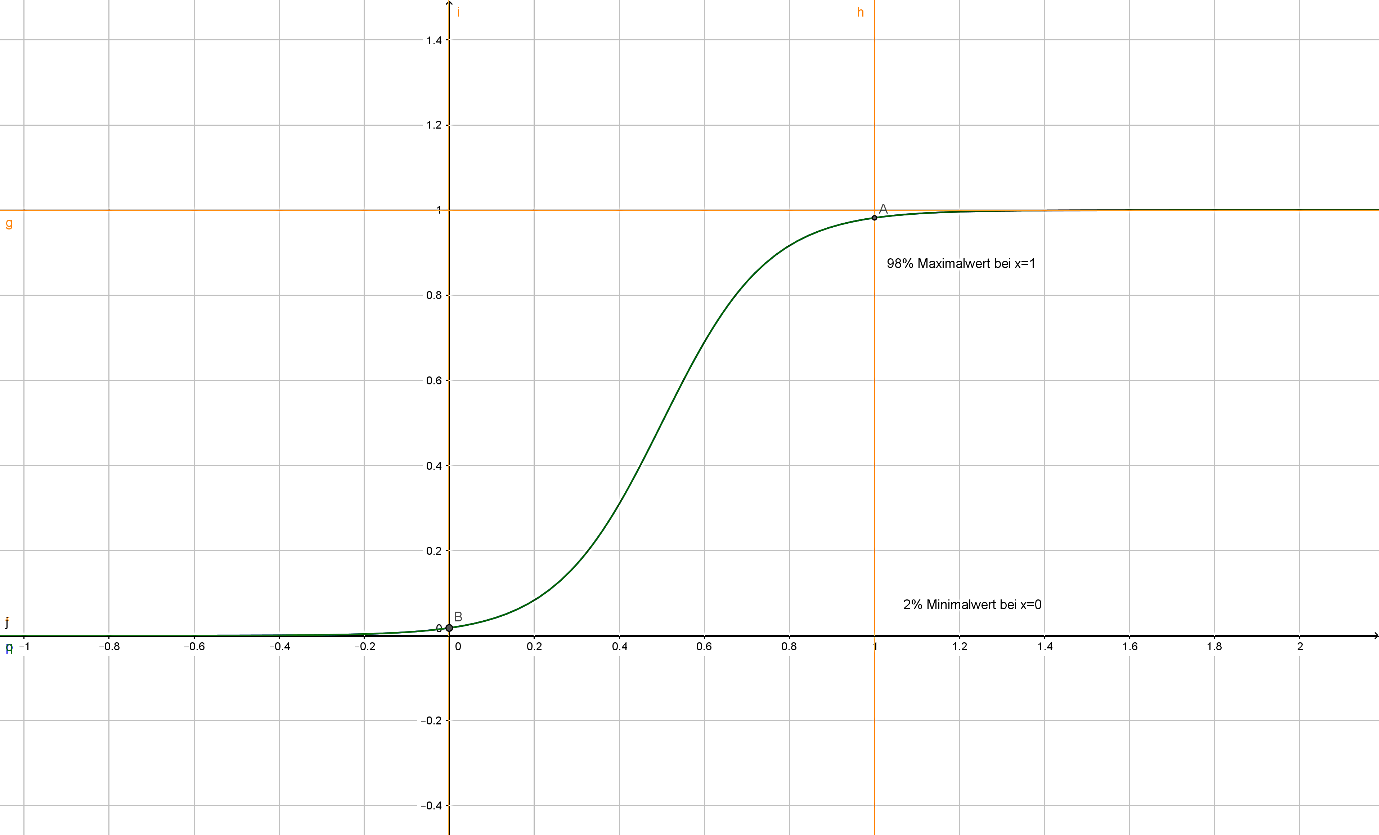
\includegraphics{Funktion.png}
	\caption{Grafik der Hyperbolischen Funktion}
	\label{hyperbolic_function}
\end{figure}

Im folgenden wird nun die Berechnung der Kennzahlen, sowie deren genauer Einfluss offen gelegt.  

\subsection{Marktanteil} 
Der Marktanteil eines Unternehmens zählt zur Kategorie der weichen Kennzahlen und berechnet sich einfach aus dem Verhältnis der eigenen verkauften Produkte, zu den verkauften Produkten aller Unternehmen. Diese wird dabei nicht durch die hyperbolische Funktion angepasst, da diese Kennzahl ein reines Verhältnis widerspiegelt. Des weiteren wird nicht zwischen den einzelnen Kategorien der Artikel, also ob Duffel oder Rucksack o.ä. unterschieden, da es sich um einen großen gemeinsamen Markt (den der Outdoor \enquote{Accessoires}) handelt. Dies bedeutet auch, dass wenn sich plötzlich viele neue Spieler anmelden, der eigene Marktanteil drastisch senken kann. 

Der Marktanteil besitzt keine weiterführenden Wechselwirkungen, sondern ist nur ein Indikator, wie sich das Unternehmen im Vergleich zu den anderen schlägt. Dadurch, dass die Verkaufswahrscheinlichkeit zum Großteil bestimmt, ob man Deals gewinnt und diese dann den Marktanteil bestimmen, ist es wichtig eine möglichst hohe Verkaufswahrscheinlichkeit zu besitzen um möglichst viele Deals für sich zu gewinnen, wenn man seinen Marktanteil maximieren möchte. 

\subsection{Mitarbeiterzufriedenheit}
Die Mitarbeiterzufriedenheit des Unternehmens berechnet sich aus dem Durchschnittsgehalt aller Mitarbeiter die im Unternehmen angestellt sind. Dieses wird durch einen festgelegten Wert geteilt, der benötigt wird um eine 100-prozentige Zufriedenheit der Mitarbeiter nur auf Basis ihres Gehaltes zu gewährleisten. Dieser Wert entspricht bisher 70.000\€ jährlich, da dies ein angemessener Durchschnittswert für alle Mitarbeiter, also auch die, die nur in der Produktion arbeiten, sowie für die normalerweise besser verdienenden Sales-Leute, ist, um eine volle Zufriedenheit zu erreichen. Diese kann auch durch soziale Leistungen, wie zum Beispiel dem Aufbau einer Kantine erhöht werden, sodass ein Durchschnittsgehalt von 70.000\€ nicht zwingend notwendig ist um eine vollständige Zufriedenheit der Mitarbeiter sicherzustellen. 

Eine hohe Mitarbeiterzufriedenheit hat vielerlei positive Auswirkungen auf das Unternehmen. Sie erhöht zum Beispiel die Produktivität der Mitarbeiter in der Produktion, von daher können mit derselben Anzahl Mitarbeiter mehr Produkte im Monat hergestellt werden. Außerdem bestimmt sie das Image, wodurch indirekt die Verkaufswahrscheinlichkeit erhöht wird und verkürzt die Dauer der Forschungsprojekte, da zufriedenere Mitarbeiter einfach effektiver arbeiten. 
\subsection{Kundenzufriedenheit}
Die Kundenzufriedenheit startet immer bei 0\% und lässt sich durch Forschungsmaßnahmen erhöhen. Diese geben den Produkten sozusagen neue Alleinstellungsmerkmale, die den Kunden glücklicher mit dem erworbenen Produkt werden lassen. Dies ist der einzige Weg seine Kunden zufrieden zu stellen, jedoch sinkt die Kundenzufriedenheit, wenn man gewonnene Deals nicht erfüllt, mal abgesehen von dem Verlust durch Konventionalstrafen (mehr dazu später), sowie wie die anderen weichen Kennzahlen auch in bestimmten Zeitabständen.

Die Kundenzufriedenheit spielt eine wichtige Rolle für das Image, welches neben dem Bekanntheitsgrad der ausschlaggebende Faktor in der Verkaufswahrscheinlichkeit, das heißt sie spielt auch eine relativ wichtige Rolle in dem Erfolg des Unternehmens, da Produkte verkaufen der einzige Weg Umsatz zu erzielen ist.  
\subsection{Image}
Das Image eines Unternehmens ist das generelle Bild welches Externe, also Kunden, sowie andere Unternehmer von der Firma haben. Dieses ist die erste hier aufgeführte Kennzahl, die sich nur aus anderen zuvor erklärten Kennzahlen berechnet. Sie wird zur einen Hälfte aus der Mitarbeiter- und zur anderen Hälfte der Kundenzufriedenheit berechnet, da zufriedene Mitarbeiter oder Kunden positiv von dem Unternehmen sprechen, wodurch sich das Image verbessern könnte. Außerdem haben Unternehmen von denen generell die Mitarbeiter und Kunden alle Unzufrieden sind es eher schwerer ein positives Image in der Öffentlichkeit zu bewahren. 
Das Image beeinflusst die Verkaufswahrscheinlichkeit und kann auch durch soziale Projekte, wie zum Beispiel Spenden erhöht werden.
\subsection{Bekanntheitsgrad}
Der Bekanntheitsgrad wird ähnlich wie die Kundenzufriedenheit nicht berechnet, sondern startet auch bei 0\% und erhöht sich nur durch Aktionen in der Marketing Abteilung. Er ist neben dem Image der Hauptfaktor für die Verkaufswahrscheinlichkeit, von daher ist es sehr empfehlenswert in irgendeiner Art Marketing Maßnahmen durchzuführen. 
\subsection{Verkaufswahrscheinlichkeit}
Die Verkaufswahrscheinlichkeit ist wahrscheinlich die Kennzahl mit dem größten Einfluss auf den Erfolg des Unternehmens, da es mit einer schlechten Verkaufswahrscheinlichkeit fast unmöglich ist irgendwelche Deals zu gewinnen und außerdem eine hohe Verkaufswahrscheinlichkeit auch die Erträge aus Deals erhöht. Da diese die einzige Möglichkeit sind Gewinne zu erzielen sollte man unbedingt eine hohe Verkaufswahrscheinlichkeit anstreben. Diese wird zu 50\% aus dem Image und zu den anderen 50\% aus dem Bekanntheitsgrad gerichtet, also sollte das Hauptziel jedes Unternehmers sein diese zu maximieren. Dies ist in der Realität fundiert, da ein vollkommen unbekanntes Unternehmen nur schwer Deals gewinnen kann, da niemand \enquote{No-Name} Produkte kauft. Des weiteren ist es vor allem auf einem Markt, wie dem der Outdoor Artikel sehr schwer Käufer zu finden wenn das Unternehmen ein sehr negatives Image hat, da die Käufer besonders großen Wert auf Qualität legen und lieber mehr zahlen, als zu wissen, dass ihre Produkte unter sehr schlechten Arbeitsbedingungen, zum Beispiel, hergestellt werden. 

\section{Absatz der Produkte}
Es werden durchgehend öffentliche Ausschreibungen generiert, deren Anzahl mit der Anzahl an aktiven Spielern auf dem Markt skaliert, das heißt gibt es mehr Bewerber, werden logischerweise auch mehr Ausschreibungen erstellt. Für diese hat nun jeder Spieler einen Monat (in Spielzeit), also in etwa 8 Stunden um sich darauf zu bewerben, bevor eine Entscheidung für ein Unternehmen getroffen wird. Wer aktiv ist und sich zuerst bewirbt hat eine theoretisch höhere Chance die Ausschreibung für sich zu entscheiden als spätere Bewerber, denn am Entscheidungstag wird eine Zufallszahl zwischen 0 und 1 erstellt und mit der Verkaufswahrscheinlichkeit des ersten Bewerbers verglichen. Ist die Kennzahl höher als die erzeugte Zufallszahl wird der Deal gewonnen, falls nicht wird dieselbe Rechnung mit dem nächsten Bewerber durchgeführt, bis ein Unternehmen die Ausschreibung für sich entscheidet, oder kein Bewerber mehr über ist. 

Die geforderten Produkte in den Ausschreibungen werden zufällig erstellt, sowie die Menge, jedoch im Verhältnis zur Durchschnittsproduktion aller Unternehmen und die Laufzeit variiert auch zufällig, das heißt es können Aufträge für 1000 Rucksäcke jeden Monat 2 Jahre lang oder eine Einmal-Bestellung von 500 Duffels zum Beispiel erstellt werden. Ist ein Deal einmal gewonnen, kann dieser nicht mehr abgebrochen werden und Nichtlieferung führt zu Konventionalstrafen in Höhe von 75\% des Preises. Dieser wird nach Gewinn des Deals berechnet, da die Kennzahl Verkaufswahrscheinlichkeit auch eine Rolle bei der Höhe des erzielten Gewinnes spielt, da Unternehmen mit einem besseren Image oder höherem Bekanntheitsgrad, höhere Preise erzielen können. 

\section{Jahresabschluss} \label{Jahresabschluss}
Nach dem Handelsgesetzbuch (HGB) sind alle Kaufleute verpflichtet, einen Jahresabschluss aufzustellen (vgl. § 242 HGB). Dieser besteht aus Bilanz und GuV, Kapitalgesellschaften müssen zusätzlich einen Anhang, sowie Lagebericht veröffentlichen. Der Jahresabschluss hat unter anderem eine Dokumentationsfunktion,gekennzeichnet durch eine laufende Buchführung, sowie eine Informationsfunktion.Letztere ermöglicht einen Überblick über die Vermögenslage (Mittelverwendung), die Finanzlage (Mittelherkunft) und die Ertragslage eines Unternehmens.
In unserem Planspiel werden in der Bilanz und der GuV nur die in diesem Spiel berührten Positionen aufgeführt, welche den beim Kennzahlenprinzip erwähnten \enquote{harten} Kennzahlen entsprechen. Einmal jährlich wird ein Jahresabschluss durchgeführt um die Bilanz auszugleichen. 
Im Spiel wird auch unterjährig eine nicht ausgeglichene Bilanz angezeigt, welche aber nicht zur Veröffentlichung, sondern nur zur Information des Spielers dient. Diese enthält die in diesem Spiel berührten Aktiv- und Passiv-Positionen: 
\begin{itemize}
\item \textbf{Aktiva}	
	\begin{itemize}
		\item Technische Anlagen und Maschinen
		\item Gebäude
		\item fertige Erzeugnisse
		\item liquide Mittel
	\end{itemize}
\item \textbf{Passive}
	\begin{itemize}
		\item Fremdkapital
		\item Eigenkapital
	\end{itemize}
\end{itemize}

Jeder Spieler beginnt mit einem Eigenkapital von 100.000€ und von daher auch mit liquiden Mitteln in der selben Höhe. Die restlichen Bilanzpositionen entsprechen erst einmal 0 und können zum Beispiel durch den Kauf von Produktionsmaschinen oder Lager- beziehungsweise Produktionshallen erhöht werden. Die fertigen Erzeugnisse werden direkt durch Produktion und dadurch Senkung der liquiden Mittel erhöht, da wir keine eigenen Rohstoffkonten haben und von daher direkt produziert wird wenn man Geld für die Herstellung ausgibt. Außerdem lassen sich die Liquiden Mittel durch Aufnahme von Krediten, also Fremdkapital aufstocken.

Die Gewinn- und Verlustrechnung erhält auch nur die Aufwands- und Ertragsposten die in unserer Simulation relevant sind und diese beschränken sich auf:
\begin{itemize}
	\item \textbf{Aufwendungen}	
	\begin{itemize}
		\item Aufwendungen für Rohstoffe
		\item Aufwendungen für Werbung
		\item Aufwendungen für Gehälter
		\item Aufwendungen für Energie
		\item Aufwendungen für soziale Leistungen
		\item Zinsaufwendungen
		\item Aufwendungen für Fremdinstandhaltung
		\item Schadensersatzzahlungen
		
	\end{itemize}
	\item \textbf{Erträge}
	\begin{itemize}
		\item Umsatzerlöse für fertige Erzeugnisse
		\item Jahresüberschuss
	\end{itemize}
\end{itemize}

Unsere GuV enthält alle Aufwandskonten die in unserer Simulation möglicherweise belastet werden könnten und außerdem das einzige Ertragskonto, die Umsatzerlöse, die wie schon mehrfach erwähnt wurde unsere alleinige Umsatzquelle sind. Der Jahresabschluss wird einmal jährlich aus den Umsatzerlösen - die kumulierten Aufwendungen berechnet und danach entweder dem Eigenkapital in der Bilanz zugerechnet (wenn die Erlöse höher sind als die Aufwendungen) oder vom Eigenkapital substrahiert, wenn er negativ ist. Dadurch erhält der Spieler einen guten Überblick über den Erfolgs des Unternehmens der letzten Quartale und erhält außerdem einen Indikator auf seine Chancen in der Highscore Liste zu landen, da dort das Eigenkapital übernommen wird, also der kumulierte Gewinn seiner 10 Jahre Spielzeit. 

\section{Abteilungen}
\subsection{Einführung}
Es gibt in diesem Planspiel sechs verschiedene Abteilungen, denen der Spieler Mitarbeiter zuordnen und in denen er freie Entscheidungen treffen kann. Diese Abteilungen, sowie die einzelnen Entscheidungsmöglichkeiten und deren Konsequenzen werden in diesem Kapitel erklärt. Außerdem wird die Funktion der Mitarbeiter, die den einzelnen Abteilungen unterstellt sind erläutert und die Hintergründe beleuchtet, warum man Mitarbeiter in bestimmten Abteilungen einstellen muss.
\subsection{Human Ressources}
Über die Abteilung Human Ressources ist es dem Spieler möglich neue Mitarbeiter einzustellen und deren Abteilung, sowie Gehalt zu bestimmen. Dieses ist vollkommen frei wählbar und daher sind dem Unternehmer alle Möglichkeiten offen eine bestimmte Führungsstrategie zu verfolgen, wie etwa Kostenführerschaft, durch möglichst geringe Gehaltszahlungen und Produktionskosten. Jedoch wirkt sich das Gehalt direkt auf die Mitarbeiterzufriedenheit und dadurch einige andere Kennzahlen des Unternehmens aus. Weiterhin lassen sich dort die derzeitigen Mitarbeiter einsehen und der Spieler kann soziale Projekte starten, wie zum Beispiel einen Kindergarten für die Mitarbeiterkinder eröffnen, freies WiFI einrichten, Urlaubs- oder Weihnachtsgeld zusätzlich ausbezahlen oder eine Kantine finanzieren. Dadurch erhöht sich die Mitarbeiterzufriedenheit deutlich, jedoch sind alle diese Leistungen auch mit monatlichen, beziehungsweise einmaligen Kosten verbunden. Außerdem ist für jeden 10. Mitarbeiter den man generell einstellen möchte, ein Mitarbeiter, der der Abteilung Human Ressources unterstellt ist notwendig, da man ab einer gewissen Größe des Unternehmens die Mitarbeiter nicht mehr alleine einstellen und verwalten kann. 

\subsection{Produktion}
In der Produktionsabteilung kann der Unternehmer, wie der Name schon sagt, Produkte herstellen. Dafür muss er eine Lager-, sowie Produktionshalle erwerben, mindestens einen Mitarbeiter in dieser Abteilung einstellen und eine Produktionsmaschine kaufen, für den Artikel den er gerne herstellen würde. Die monatliche Produktionsmenge kann vom Spieler in vorm von Produktlinien festgelegt werden, sofern die eben genannten Grundvoraussetzungen erfüllt sind. Die maximale Produktionsmenge pro Monat wird durch die Anzahl der Maschinen, welche hingegen vom Platz in der Produktionshalle beschränkt ist, und der Anzahl der Mitarbeiter festgelegt. Der niedrigere Wert von beidem bestimmt die Obergrenze, wobei die maximalen Produkte pro Monat pro Mitarbeiter durch eine hohe Mitarbeiterzufriedenheit erhöht werden kann, da sehr zufriedene Mitarbeiter mit den selben Maschinen mehr produzieren können, da sie weniger Fehler machen.

Der Spieler hat die Auswahl Produkte der drei verschiedenen Qualitätsstufen A, B und C herzustellen. Die jeweiligen Herstellungskosten basieren auf Einkaufskosten der verschiedenen Produkte von wirklichen Outdoorherstellern um die Hälfte reduziert, da in unserem Planspiel nur die Herstellungskosten gefordert sind und Aufwendungen wie Energie oder die Maschinen (die in den Kaufpreis logischerweise eingerechnet sind) oder Gewinnmargen noch heruntergerechnet werden müssen. 

Die Grundvorraussetzungen für die Produktion sind sehr komplex, jedoch von der Realität ableitbar, da man ohne Halle zum Beispiel nur schwer produzieren kann und die jeweiligen Funktionen zum Kaufen der einzelnen Bestandteile sehr offensichtlich in der Produktionsabteilung ersichtlich sind.

\subsection{Forschung}
Auf dem Outdoor Markt spielt die Weiterentwicklung der eigenen Produkte eine große Rolle um die eigene Marktpositionen zu stärken und dies kann man in der Abteilung Forschung durchführen. Es gibt zwei verschiedene Arten durchführbarer Forschungen, beide für alle verschiedenen Produktqualitätsstufen differenziert. Der Spieler kann die Kundenzufriedenheit seiner Produkte verbessern, indem er nach neuen Zusatzfeatures forscht, die das Erlebnis der Kunden mit dem Produkt besser machen und dadurch die Zufriedenheit erhöhen oder durch die Erforschung neuer Produktionsmethoden die Herstellungskosten für ein bestimmtes Produkt in einer bestimmten Qualitätsstufe senken, um sich so weiter auf eine bestimmte Produktion zu spezialisieren. Um eine Forschung durchführen zu können, muss mindestens ein Mitarbeiter in der Forschungsabteilung eingestellt werden und die Zeit die ein einziges Forschungsprojekt dauert, skaliert mit der Anzahl der Mitarbeiter die daran arbeiten, das heißt je mehr Mitarbeiter man in der Abteilung einstellt, desto schneller werden Forschungen abgeschlossen. Weiterhin beschleunigt werden diese durch zufriedene Mitarbeiter. 
Diese Abteilung stellt die einzige Möglichkeit dar, die Kundenzufriedenheit zu erhöhen und ist damit sehr relevant für die Verkaufswahrscheinlichkeit.

\subsection{Marketing}
In der Marketingabteilung kann der Unternehmer Marketingkampagnen starten um seine Produkte zu bewerben und so den Bekanntheitsgrad seines Unternehmens zu erhöhen, um die Chance Deals zu gewinnen zu steigern. Es gibt vier verschiedene Kampagnen mit unterschiedlichen Kosten und dementsprechenden benötigten Mitarbeitern um diese durchzuführen. Diese sind eine den Kosten nach aufsteigend sortiert \enquote{Sozial Media Kampagne}, \enquote{Werbung in Printmedien}, \enquote{Radiowerbespot} und \enquote{TV-Spot}. Die im Interface angezeigten Kosten werden täglich abgerechnet und entsprechen realen Kosten, für die Simulation der Kosten für einen TV-Spot zum Beispiel wurden einige Berechnungsannahmen getroffen. Die 130.000 \€ täglich setzen sich aus den generellen Sendekosten an den Sender (ca 60.000 pro Spot in der Prime-Time, je nach Sender) und den Produktionskosten für einen eigenen Spot zusammen. Diese werden nicht als direkte Fixkosten abgerechnet, sondern gehen in den täglichen Kosten auf. Weiterhin wird davon ausgegangen, dass der Spot zwei mal täglich in der \enquote{Prime-Time} gesendet wird, um so die größtmögliche Zielgruppe zu erreichen und dem Spieler, mit schon hohen Einnahmen eine Möglichkeit zu geben seine Verkaufsmöglichkeiten enorm zu erhöhen. Außerdem werden mindestens 7 Mitarbeiter in der Abteilung Marketing benötigt um einen Tv-Spot zu ermöglichen. 

\subsection{Finanzen}
Die Finanzabteilung bietet Einsicht in die vorher erklärte Bilanz und GuV des Unternehmens und gibt so dem Spieler einen Überblick über seinen Erfolg und seine laufenden Kosten. Außerdem bietet diese Abteilung die Möglichkeit Kredite aufzunehmen um so die Zahlungsmittel des Unternehmens zu erhöhen. Die Zinsen für den Kredit werden mithilfe der Verschuldungsquote, also Eigenkapital / Fremdkapital berechnet. Überschreitet diese zwei, hat man also doppelt so viel Fremdkapital wie eigenes ist es nicht mehr möglich neue Kredite aufzunehmen, da der Bank nicht genug Sicherheiten angeboten werden können, um einen neuen Kredit gewährt zu bekommen.

\subsection{Vertrieb}
In der Abteilung Vertrieb kann der Spieler die derzeit offenen Ausschreibungen sehen und sich darauf bewerben, außerdem werden die gewonnenen Deals mit Auftragsvolumen angezeigt, wodurch man sich einen Überblick darüber verschaffen kann, wieviel man diesen Monat produzieren muss um seine Verträge zu erfüllen. Jedes Unternehmen beginnt bei Erzeugung direkt mit einem zufällig generierten Auftrag, ohne Konventionalstrafe um dem Spieler direkt einen schnellen Start mit Aussicht auf Gewinne zu ermöglichen, ohne einen Monat nur zu produzieren und zu hoffen man gewinnt einen der ersten Deals. Des weiteren erfolgt in dieser Klasse die in diesem Kapitel erklärte Ausschreibungsgewinnermittlung. Um sich auf neue Ausschreibungen bewerben zu können, muss man mindestens einen freien Mitarbeiter besitzen, da jeder Mitarbeiter der einen langfristigen Deal gewonnen hat, sich vollkommen auf diese Firma fokussiert um den Kunden aktiv zu betreuen und Folgeaufträge zu generieren. 

\section{Gewinnermittlung}
Dadurch das unsere Simulation Echtzeitbasiert ist und immer neue Mitspieler auf den Markt auftreten gibt es nie einen wirklichen Gewinner, sondern die Spieler können sich nur durch abschließen des Spiels mit möglichst hohem Eigenkapital, also kumulierten Gewinnen über ihre 10 Jahre Spielzeit einen Platz in der High-Score-Liste sichern. Spieler die vor Ende ihrer 10 Jahre Führungszeit bankrott gehen, werden nicht in die in die Liste aufgenommen.

\section{Zusammenfassung}
In diesem Kapitel wurden die Grundlagen für die Erstellung eines realistischen Planspiels gelegt. Es wurden für dieses Spiel spezifische Kennzahlen und wirtschaftliche Hintergründe, sowie deren Berechnungen erläutert. Deren Wechselwirkungen sollen zu einem einzigartigen Spielerlebnis beitragen und die einzelnen Abteilungen erlauben eine Vielfalt an Entscheidungsmöglichkeiten und verschiedenen Führungsstrategien. Im nächsten Kapitel wird auf den Entwurf und die Architektur unseres Spiels eingegangen.
\chapter{Entwurf}
\section{Konzept \textnormal{\textsf{\small{Niklas Schuster}}}}
\subsection{Spieldynamik}
Die Spieldynamik des zu entwickelnden Planspiels wird gesteuert und bestimmt durch ein Double-Layer Ansatz welcher das Kernelement des Spiels darstellt und folgende logische Schichten beinhaltet:
\begin{enumerate}
\item Die erste Schicht beinhaltet sämtliche funktionale Spielinhalte wie die einzelnen Abteilungen und Features, die für die Spieler spielbar sind.
\item Die zweite Schicht umfasst ein umfangreichen Zahlenpool, welcher aus monetären und nicht monetären Kennzahlen besteht und bestimmt ist die Entscheidungen des Spielers effektiver und realistischer auf das Spielgeschehen abzubilden.
\end{enumerate}
Entscheidend hierbei ist, dass jede Aktion im Spiel die der Spieler ausführt direkten Einfluss auf den Erfolg des zu führenden Unternehmens hat. Dies wird an folgendem Beispiel deutlich:
\par In der Abteilung Human Ressource hat der Spieler die Möglichkeit Mitarbeiter für sein Unternehmen einzustellen. Ein Mitarbeiter ist im Spiel ein Objekt welches verschiedene Attribute aufweist. So bekommt ein Mitarbeiter z.B. ein Gehalt, sowie eine Abteilung die ihm vom Spieler zugewiesen beziehungsweise als Eingabe durch den Spieler frei wählbar ist. Das Gehalt was den Mitarbeitern bezahlt wird beeinflusst der Höhe nach die Kennzahl Mitarbeiterzufriedenheit und andere Kennzahlen aus dem Zahlenpool beeinflusst. Der Durchschnitt aller Kennzahlen ist ein Indikator für die Marge die sich beim Verkauf von Produkten entsteht. Ein Unternehmen mit zufriedenen Mitarbeitern und einem guten Image kann also Produkte zum selben Herstellungspreis teurer Verkaufen. Somit ergeben sich automatisch aus dem Führungsstil des Spielers unterschiedliche Unternehmensstrategien wie die Kostenführerschaft oder Differenzierung. Wenn der Spieler nur einen geringen Durchschnitt aller Kennzahlen erzielt, weil er z.B. seinen Mitarbeitern wenig Geld zahlt und folglich eine geringere Marge erhält, bleibt ihm nur die Möglichkeit seine Produkte billig zu produzieren und durch hohe Absatzmengen erfolgreich zu sein (Kostenführerschaft). Andersherum wäre es effektiver teuer zu produzieren (Differenzierung). Die Abteilung die den Mitarbeitern zugewiesen wird beeinflusst ebenfalls drastisch das Spielgeschehen. Durch viele im Sales beschäftigte Mitarbeiter steigt beispielsweise die Chance einen Deal zu gewinnen und die maximale Anzahl an Kunden die gleichzeitig betreut werden können usw. So lässt sich allein durch das Einstellen von Mitarbeitern sein Unternehmen bewusst in eine bestimmte Richtung steuern.
\par Mit diesem Konzept wird ein Ansatz verfolgt bei dem der Spieler im Verhältnis ein begrenztes Maß an Aktionen ausführen kann, wodurch das Planspiel übersichtlich und intuitiv für den Spieler bleib, aber gleichzeitig durch das Kennzahlen Modell ein hohes Maß an Komplexität und Entscheidungsfreiheit geschaffen wird. Somit kann im Early-Game der Start für den Spieler erleichtert werden und im Mid/End-Game weiterhin erfolgsrelevante Entscheidungen getroffen werden.

\subsection{Echtzeit \& Ranking}
Um die Entscheidungen im Spiel noch erfolgsrelevanter gestalten zu können wird im Spiel auf ein "Echtzeit" System gesetzt. Die Zeit In-Game basiert auf einem Datumssystem wobei ein Tag 16 Minuten in Real-Time entspricht. Die gesamte Spielzeit des Spiels ist beschränkt auf 10 Geschäftsjahre, dabei ist es irrelevant zu welcher Zeit der Spieler mit dem Spiel beginnt. Sobald sich ein Spieler auf dem Server registriert beginnt seine Spielzeit. Nach den 10 Geschäftsjahren ist das Spiel für den jeweiligen Spieler beendet und sein Unternehmen wird in eine Highscoreliste eingetragen. Somit lässt sich das Spiel unabhängig von anderen Spielern frei spielen, wobei sich der Markt und die Konkurrenzsituation aus allen momentan aktiven Spielern ergibt. Durch das Login System ist die Spieleranzahl beliebig skalierbar. Der Faktor der Zeit spielt im Spiel eine Entscheidende Rolle und hebt den planerischen Aspekt des Spiels deutlicher hervor, hierzu ein Beispiel:
\par In der Produktion können Maschinen für die Herstellung von Produkten gekauft werden. Diese haben eine maximale Ausbringungsmenge, welche pro Monat angegeben wird: in diesem Beispiel 30.000 Einheiten pro Monat. Die tatsächlich produzierte Menge werden aber pro Tag ausgeschüttet, was einer Menge von 1.000 Einheiten entspricht die dem Warenlager hinzugefügt werden (Ausgegangen von 30 Tagen im Monat). Das Lieferdatum gegenüber aktiven Kunden ist in den Verträgen immer zum Ende des Monats angesetzt. Momentan ist eine Ausschreibung offen zum 15. des Monats, wobei der Kunde jeweils 50.000 Einheiten pro Monat beziehen will. Der Bestand im Warenlager beläuft sich am 15. des Monats ebenfalls auf 30.000 Einheiten. An dieser Stelle muss der Spieler neben der entstehenden Kosten auch den Faktor der Zeit deutlich in seine Überlegung mit einbeziehen:
\begin{itemize}
   \item Wie viel produziert meine Maschine in den verbleibenden Tagen bis Monatsende?
    \item Ist dann durch den Lagerbestand die Bezugsmenge des Kunden gedeckt?
    \item Kann die Bezugsmenge des Kunden in der verbleibenden Zeit durch eine zusätzliche Maschine gedeckt werden?
    \item Können die dadurch entstandenen Mehrkosten getragen werden?
\end{itemize}
\par Außerdem kann durch den Ansatz einer Echtzeit Simulation zusätzlich das unternehmerische Risiko erhöht werden, wie z.B. Konventionalstrafen bei Nichterfüllung der auszuliefernden Mengen an den Kunden. Spieler die aktiver am Markt sind können sich so ebenfalls einen Zeitvorteil verschaffen, da Spieler die sich eher auf eine Ausschreibung bewerben auch bessere Chancen haben einen Deal für sich zu entscheiden.

\section{Architektur \textnormal{\textsf{\small{Markus Böbel}}}}
\label{sec:architektur}
Durch das Echtzeit-Spielkonzept des Planspiels ist es für die Anwendung von Nöten ständig Daten, auszuwerten und zu berechnen. Damit diese Berechnungen erfolgreich durchgeführt werden können, müssen diese unabhängig von der Präsenz der Spieler durchgeführt werden. Dies wird erreicht durch die Einrichtung eines einfachen verteilten Systems, indem die Programmlogik auf einem abgeschlossenen Server liegt, während sich die Spieler lediglich nötige Information anfragen oder ihr Handeln dem Server mitteilt.
Wenn nun ein Spieler das Spiel für eine gewisse Zeit unterbricht, können andere Spieler in dieser Zeit das Spiel fortführen.

Als der Software Architektur liegt ein eine einfache Three-Tier-Architektur. (siehe Abbildung \ref{abb:architektur})
Wie der Name es vermuten lässt, besteht eine solche Architektur aus drei grundlegenden Elementen.

\begin{description}
	\item[Datenschicht] Die Datenschicht dient der Datenpersistenz und besteht meist aus einer Datenbank.
	\item[Logikschicht] Diese Schicht bearbeitet die Daten der Datenschicht und bringt diese in einen semantischen Zusammenhang. 
	\item[Präsentationsschicht] Bei dieser Schicht werden die hergerichteten Daten der Logikschicht präsentiert. Sie stellt sozusagen die Schnittstelle zum späteren Spieler da, weil dieser bloß auf der Präsentationsschicht handelt.
\end{description}
Der Grund für diese Schichtentrennung ist die einfachere Austauschbarkeit der verschiedenen Bestandteile. Wenn zum Beispiel das Datenbanksystem erneuert werden soll, so ist dies ohne großen Aufwand möglich. Das Gleiche gilt auch für die anderen Bestandteile.

Im konkreten Falle des Planspiels besteht die Präsentationsschicht aus einer Webseite. Diese sendet die Eingaben des Benutzers weiter an eine REST-Schnittstelle (siehe Kapital \ref{sec:rest}). Diese wird auf einem Tomcat Server initialisiert, auf welchem die Anfragen bearbeitet und das Spielkonzept umgesetzt werden.


\begin{figure}[h]
	\centering	\includegraphics[width=\textwidth]{img/architektur}
	\captionsetup{format=hang}
	\caption{
		\label{abb:architektur}Aufbau der Applikationsarchitektur}
\end{figure}

 Auf die Datenschicht wird im Falle des Planspiels verzichtet, da es keine Voraussetzung die Daten persistent zu halten und dies einen hohen Mehraufwand darstellen würde. Daraus folgt, dass die Daten nun zur Laufzeit bearbeitet und verwaltet werden.
 Im Falle eines Serverneustartes oder -ausfalls würden folglich alle Planspieldaten wie zum Beispiel Spielstände verloren gehen. Da aufgrund von Wartungsarbeiten Serverneustarts nichts Ungewöhnliches ist und es sich bei dem Planspiel um ein langwieriges Spiel handelt, ist es von Nöten eine Datenschicht nachträglich zu implementieren. 

\section{Programmentwurf \textnormal{\textsf{\small{Christian Sasse}}}}

\subsection{Use-Case-Diagramm}
In Use-Case-Diagrammen wird das externe Systemverhalten aus Anwendersicht beschrieben. Sie stellen das geplante System, die Akteure, die Verwendung des geplanten Systems (Anwendungsfälle) und die Beziehungen zwi­schen Akteuren und Anwendungsfällen dar. Kurz gesagt: Use Case Diagramme geben Auskunft darüber, was ein geplantes System aus Sichtweise der Benutzer leisten soll. In dem in dieser Arbeit behandelten Planspiel soll das Use Case Diagramm zeigen, was der Akteur, also der Spieler, alles steuern kann.
Das Use-Case Diagramm besteht aus folgenden Elementen:

\begin{description}
\item[Use Case (Anwendungsfall)]
 Ein Anwendungsfall ist ein in sich abgeschlossener Vorgang, der für einen oder mehrere Akteure ein beobachtbares Ergebnis liefert. Er beschreibt aus Sicht der Akteure welche Leistungen das System für den Anwender zur Verfügung stellt. Ein Use Case stellt somit einen Teil der Gesamtfunktionalität des Systems dar. es wird durch eine Ellipse dargestellt. 

\item[Akteur]
Der Akteur ist ein Element, das nicht zum geplanten System gehört. Er kann eine Person sein, die auf das System zugreift, oder ein anderes System, das mit dem geplanten System kommuniziert. In diesem Planspiel ist der Akteur somit der Spieler und wird als Strichmännchen dargestellt.

\item[Assoziation]
Eine Linie stellt eine Assoziation zwischen einem Akteur und einem Use Case dar. Sie beschreibt den Zugriff des Akteurs auf die Funktionalität, die das System in diesem Use Case zur Verfü­gung stellt, bzw. eine Antwort des Systems an einen Akteur. In Abbildung \ref{abb:use_case_assoziation} wird eine solche Assoziation dargestellt. dort ist zu sehen, dass der Akteur einen Mitarbeiter einstellen kann.
\begin{figure}[h]
	\centering	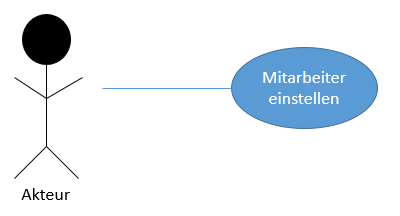
\includegraphics[width=0.5\textwidth]{img/programmentwurf/use_case_assoziation}
	\captionsetup{format=hang}
	\caption{
		\label{abb:use_case_assoziation}Assoziation in einem Use-Case-Diagramm}
\end{figure}

\item[Include-Assoziation]
Bei der Include-Beziehung verwendet ein Use Case die Funktionalität, die ein anderer Use Case zur Verfügung stellt. Der inkludierte Use Case wird immer ausgeführt. Dies ist in Abbildung \ref{abb:use_case_include} zu sehen. Hier ist zu erkennen, dass der von dem Akteur eingestellte Mitarbeiter einer Abteilung zugewiesen wird.



\begin{figure}[h]
	\centering	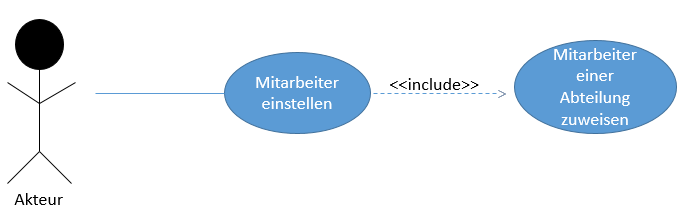
\includegraphics[width=0.5\textwidth]{img/programmentwurf/use_case_include}
	\captionsetup{format=hang}
	\caption{
		\label{abb:use_case_include}Include-Assoziation}
\end{figure}

\item[Extend-Assoziation]
Die Extend Beziehung, beschreibt die Erweiterung der Funktionalität eines Use Cases durch einen anderen Use Case. Man kann dadurch optionales Verhalten beschreiben, bzw. Funktionen modellieren, die nur unter bestimmten Bedingungen ausgeführt werden. Die folgende Abbildung zeigt eine solche Beziehung, wie sie im Planspiel auftritt. Der Akteur hat die Wahl, den Bestand der zu produzierenden Produkte zu verändern.
\begin{figure}[h]
	\centering	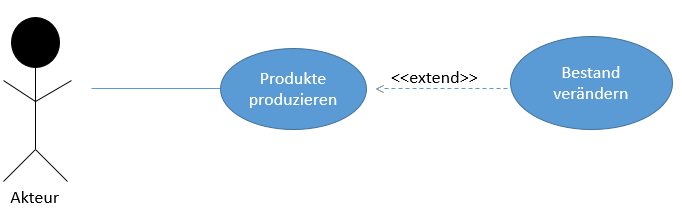
\includegraphics[width=0.5\textwidth]{img/programmentwurf/use_case_extend}
	\captionsetup{format=hang}
	\caption{
		\label{abb:use_case_extend}Extend-Assoziation}
\end{figure}

\end{description}

Neben den oben genannten Use Cases, soll es dem Spieler, wie in Abbildung \ref{abb:usecase} zu sehen, weiterhin möglich sein Produkte zu erforschen. Nach Abschluss eines Forschungsprojektes stehen verbesserte Produkte zur Verfügung.
Ein weiterer Anwendungsfall soll das Durchführen einer Markforschung sein. Hierdurch können zum Beispiel Zielgruppen besser angesprochen werden, wodurch sich Produkte besser verkaufen lassen.

 
\begin{figure}[h]
	\centering	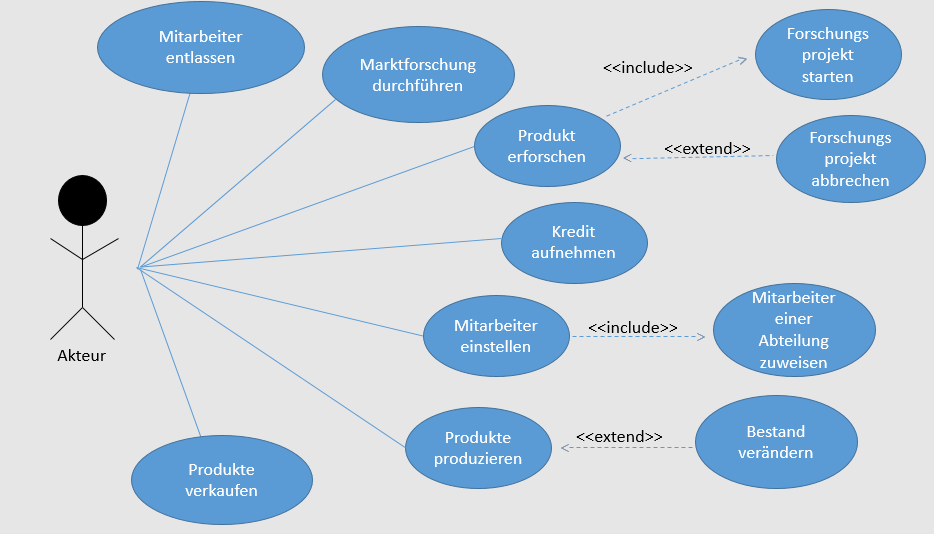
\includegraphics[width=0.5\textwidth]{img/programmentwurf/usecase}
	\captionsetup{format=hang}
	\caption{
		\label{abb:usecase}Use Case Diagramm}
\end{figure}


\subsection{Klassendiagramm}

Um die Zusammenhänge zwischen den Klassen sowie deren Aufbau zu veranschaulichen, wird ein Klassendiagramm verwendet.
Ein Klassendiagramm ist ein Strukturdiagramm der Unified Modeling Language (UML) zur grafischen Darstellung (Modellierung) von Klassen, Schnittstellen sowie deren Beziehungen.

Als \enquote{Kopf} des Planspiels dient die Klasse \texttt{Game}. Hier werden die verschiedenen Unternehmen der Spieler gelistet und die Spielzeit gesetzt und verwaltet. 

\begin{figure}[h]
	\centering	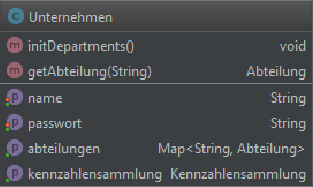
\includegraphics[width=0.5\textwidth]{img/programmentwurf/unternehmen_klasse}
	\captionsetup{format=hang}
	\caption{
		\label{abb:unternehmen_klasse}Aufbau der Klasse \enquote{Unternehmen}}
\end{figure}

In Abbildung \ref{abb:unternehmen_klasse} ist der typische Aufbau einer Klasse in UML zu sehen. Diese werden in die drei Rubriken - Klassenname, Attribute, Operationen - jeweils durch eine horizontale Linie aufgeteilt.

Die Attribute einer Klasse werden mit ihrem Namen aufgeführt und enthalten zusätzlich Angaben zu ihren Eigenschaftswerten. Methoden werden ebenfalls mit ihrem Namen, zusätzlich mit möglichen Parametern und dem Rückgabewert notiert. 

Betrachtet man die oben abgebildete \texttt{Unternehmen}-Klasse, sieht man dass dort der Name und das Passwort eines Unternehmens gesetzt werden und dessen Abteilungen und Kennzahlensammlung als Attribute enthalten sind.
Die Methode \texttt{initDepartments()} dient zum Initialiseren der Abteilungen.

Die Beziehungen zwischen den Klassen werden durch vier verschiedene Arten verdeutlicht:

\begin{description}
	\item[Assoziation]
	Beschreibt eine Beziehung zwischen zwei oder mehr Klassen. An den Enden von Assoziationen sind häufig Multiplizitäten vermerkt. Diese drücken aus, wie viele dieser Objekte in Relation zu den anderen Objekten dieser Assoziation stehen.
	\item[Aggregation (Teil-eines-Ganzen-Beziehung)]
	Liegt dann vor, wenn zwischen den Objekten der beteiligten Klassen eine Beziehung besteht,	die sich als \enquote{ist Teil von} oder \enquote{besteht aus} beschreiben lässt, also ein Objekt aus Teil-Objekten besteht.
	\item[Komposition]
	Ist eine starke Form der Aggregation und bildet den Fall ab, bei dem die Teile nicht ohne das Ganze existieren können. 
	
	Abbildung \ref{abb:unternehmen_abteilung_beziehung} stellt eine solche Beziehung dar. Die in Abbildung \ref{abb:unternehmen_klasse} gezeigte \texttt{Unternehmen}-Klasse erhält nun eine Teilklasse namens \enquote{Abteilung}, welche ohne das Unternhemen nicht existieren kann.
		\begin{figure}[h]
		\centering	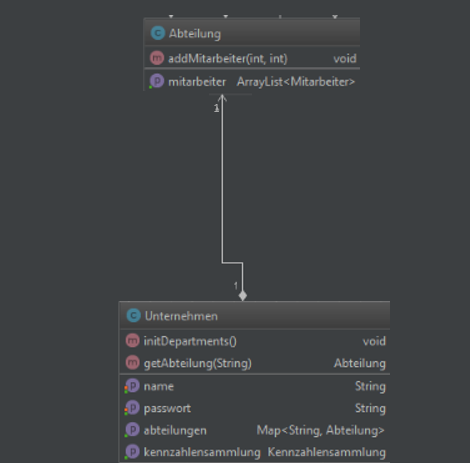
\includegraphics[width=0.5\textwidth]{img/programmentwurf/unternehmen_abteilung_beziehung}
	\captionsetup{format=hang}
	\caption{
		\label{abb:unternehmen_abteilung_beziehung}Beziehung der Klassen \enquote{Unternehmen} und \enquote{Abteilung}}
	\end{figure}

	Somit herrscht auch zwischen der \texttt{Game}-Klasse und der \texttt{Unternehmen}-Klasse eine Komposition, da es ohne das Game kein Unternehmen geben würde.
	
	\item[Create-Abhängigkeit]
	Hier erzeugt ein abhängiges Element Exemplare des unabhängigen Elementes. 
	Dargestellt wird eine dies durch einen mit \texttt{<<create>>} beschrifteten, gestrichelten Pfeil, wobei der Pfeil vom abhängigen auf das unabhängige Element zeigt.
	Durch die oben erwähnte \texttt{initDepartments()}-Methode der \texttt{Unternehmen}-Klasse, geht diese eine solche Abhängigkeit mit den gesamten Abteilungen des Unternehmens ein.
		
	\item[Generalisierung (Ist-ein-Beziehung)]
	Liegt dann vor, wenn zwischen den Objekten der beteiligten Klassen eine Beziehung besteht, die sich als \enquote{ist ein} beschreiben lässt. Das heißt, es existiert eine generellere und eine speziellere Klasse. Exemplare der spezielleren Klasse sind damit auch Exemplare der generelleren Klasse. Konkret bedeutet dies, dass die speziellere Klasse über alle Merkmale (Struktur- und Verhaltensmerkmale) der generelleren Klasse verfügt.

	Die folgende Abbildung \ref{abb:abteilungen} zeigt die Abteilungsklasse, welche als generelle Klasse dient, mit ihren spezielleren Klassen, den einzelnen Abteilungen des Unternehmens.
	\begin{figure}[h]
		\centering	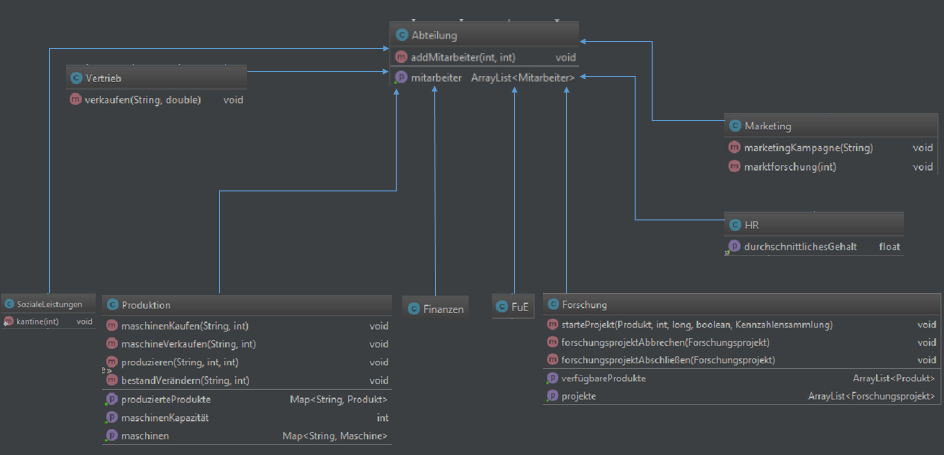
\includegraphics[width=0.57\textwidth]{img/programmentwurf/abteilungen}
		\captionsetup{format=hang}
		\caption{
			\label{abb:abteilungen}Abteilungen der Klasse \enquote{Abteilung}}
	\end{figure}	
\end{description}

Die eben gezeigte Generalisierung findet deshalb Anwendung, weil es für die Mitarbeiter der einzelnen Abteilungen noch eine eigene Klasse gibt, die eine Komposition mit der \texttt{Abteilung}-Klasse eingeht. Über deren Methode \texttt{addMitarbeiter()} können den einzelnen Abteilungen dann Mitarbeiter hinzugefügt werden. Jede Abteilung kann dabei beliebig viele Mitarbeiter enthalten. Umgekehrt kann ein Mitarbeiter jedoch immer nur in einer Abteilung arbeiten.


Die Kennzahlen eines Unternehmens, wie Fremdkapital, Eigenkapital oder Bekanntheitsgrad werden in der
\texttt{Kennzahlensammlung}-Klasse verwaltet. Jede Kennzahl erhält hierbei ihre eigene Klasse. Da die ganzen Kennzahlen jedoch gleiche Methoden, wie z.B. \texttt{berechnen()} und gleiche Eigenschaften, wie z.B. \texttt{wert} besitzen, ist es hier auch sinnvoll eine generelle Klasse zu erstellen, die diese gleichen Methoden und Eigenschaften besitzt. Diese Klasse trägt den Namen \texttt{Kennzahl}. Zu sehen ist diese Verbindung in Abbildung \ref{abb:kennzahlen_verbindung}. Innerhalb der \texttt{Kennzahlensammlung}-Klasse werden die einzelnen Kennzahlen berechnet. In der \texttt{Unternhemen}-Klasse können diese dann abgefragt werden.
	\begin{figure}[h]
	\centering	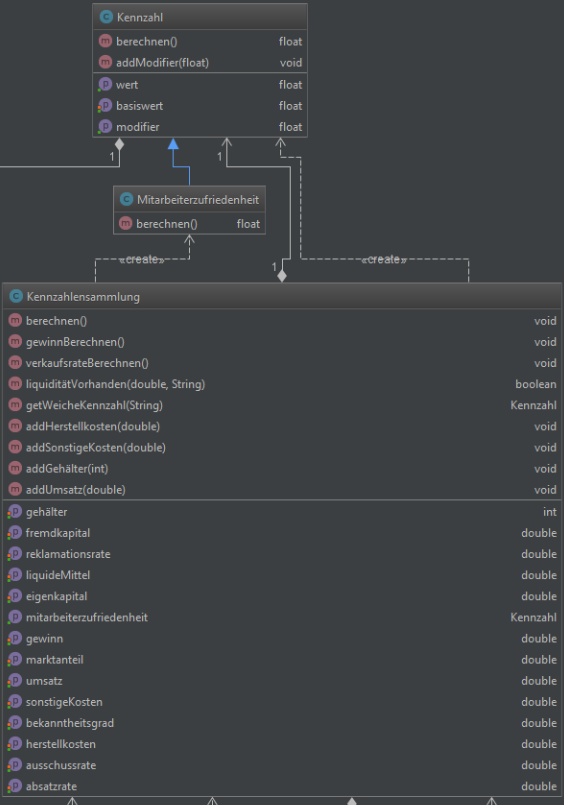
\includegraphics[width=0.5\textwidth]{img/programmentwurf/kennzahlen_verbindung}
	\captionsetup{format=hang}
	\caption{
		\label{abb:kennzahlen_verbindung}Abteilungen der Klasse \enquote{Abteilung}}
\end{figure}	

Mithilfe der Klasse \texttt{Produktion} können Produkte produziert werden. Für die Produktion werden jedoch Maschinen benötigt, die auch innerhalb der Klasse gekauft werden können. Für die Maschinen selbst gibt es wiederum eine eigene Klasse, die deren Kapazität, Klasse, Anzahl und Anschaffungskosten als Attribute enthält.
Auch für die Produkte gibt es eine eigene Klasse. Sie enthält neben dem Namen und der Anzahl auch den Preis und die Herstellungskosten als Attribute. Die \texttt{Produkt}-Klasse ist ein Teil der Produktion und könnte ohne diese nicht existieren, also herrscht hier eine Komposition. Des weiteren kann eine Produktion nur ein Produkt beinhalten. 
Produzierte Produkte können innerhalb der Klasse \texttt{Vertrieb} verkauft werden.

Die Produktforschung findet innerhalb der Klassen \texttt{Forschung} und \texttt{Forschungsprojekt} statt. 
Die Klasse \texttt{Forschung} kann hierbei beliebig viele Forschungsprojekte, gelistet im Attribut \texttt{projekte}, enthalten. Die Beziehung zwischen den beiden Klassen ist eine Komposition, da ein Forschungsprojekt ohne die Abteilung Forschung nicht existieren kann. Weiterhin kann in einem Forschungsprojekt nur ein Produkt erforscht werden. Diese Beziehung ist eine Aggregation. Ein Forschungsprojekt enthält als Eigenschaften die Dauer, das zu erforschende Produkt, den Beginn der Forschung und die Anzahl der Mitarbeiter. Man kann es starten, abbrechen und abschließen.

Die folgende Abbildung \ref{abb:klassendiagramm} zeigt das komplette Klassendiagramm. Dort sind die oben beschriebenen Beziehungen zwischen den einzelnen Klassen zu erkennen. Zu erwähnen ist, dass das Klassendiagramm nur als Grundkonzept innerhalb der Entwurfsphase dient und nicht alle Funktionen der Endanwendung widerspiegelt. Deshalb sind einige Klassen noch nicht ausgearbeitet und haben keine erkennbare Funktion. Weiterhin sind dort noch nicht alle Klassen der Kennzahlen vorhanden und es noch keine Möglichkeit seine Finanzen oder Aufträge zu verwalten.

\begin{figure}[h]
	\centering	\includegraphics[width=\textwidth]{img/programmentwurf/klassendiagramm}
	\captionsetup{format=hang}
	\caption{
		\label{abb:klassendiagramm}Vollständiges Klassendiagramm}
\end{figure}





\chapter{Entwicklung}

\section{Java Backend}

Im folgenden wird der Aufbau und die Funktionalität des Java Backends und der einzelnen Klassen dargestellt, auf Grund von Platzmangel wird hier nur auf die wichtigsten Funktionalitäten und Methoden eingegangen.

Die Klasse \enquote{Game} implementiert die Spiellogik und das Echtzeit-Konzept. Hier werden Aktionen, die alle Spieler beziehungsweise Unternehmen betreffen durchgeführt sowie die Unternehmen, beispielsweise für die Festlegung des Gewinners einer Ausschreibung, verglichen.

Die Hauptfunktionalität des Unternehmensplanspiels ist im Package \enquote{Unternehmung} umgesetzt, das, strukturell gesehen, \enquote{unter} der Klasse \enquote{Game} liegt. Hier sind neben der Klasse \enquote{Unternehmen} die einzelnen Abteilungen eines solchen mit ihren verschiedenen Möglichkeiten, die dem Spieler hier zur Verfügung stehen, implementiert (Package \enquote{Abteilungen}) sowie das Kennzahlenwesen eines Unternehmens (Package \enquote{Kennzahlen}). Darüber hinaus befinden sich in diesem Package die notwendigen Java-Klassen, durch deren Objekte ein objektorientierter Programmieransatz realisiert wird. Einige Methoden werfen Exceptions, die im Package \enquote{Exceptions} abgelegt sind.


\subsection{Die Klasse \enquote{Game}} \textnormal{\textsf{\small{Luca Dommes}}}}

In der Klasse Game ist die Logik und Mechanik des Untenehmensplanspiels implementiert, sie steht, strukturell gesehen, über allen anderen Klassen.

Zunächst einmal ist zu erwähnen, dass es sich hierbei um eine Spezialisierung der Java-Klasse \enquote{TimerTask}\footnote{https://docs.oracle.com/javase/8/docs/api/java/util/TimerTask.html} handelt. Dies dient der Umsetzung des Echtzeit-Ansatzes des Spiels. So wird im Konstruktor der Game-Klasse ein Timer-Objekt erstellt, das mit einem Intervall von 16 Minuten initialisiert wird. 16 Minuten stellen also einen Tag in Spielzeit dar. Im statischen Klassenattribut \enquote{gameCalendar} wird die Spielzeit als Calendar-Objekt\footnote{https://docs.oracle.com/javase/8/docs/api/java/util/Calendar.html} dargestellt, das bei jedem Timer Intervall einen Tag hochgezählt wird. Wenn 16 Minuten also ein Spieltag sind vergehen pro Stunde 3,75 Spieltage und dementsprechend an einem Tag (3,75 * 24 =) 90 Spieltage, sprich ein Quartal. Daraus folgt, dass ein Geschäftsjahr 4 (Echtzeit-)Tage dauert.

Die Klasse Game besteht hauptsächlich aus statischen Methoden, um die Zugriffe auf die Klasse zu erleichtern. Wie im Folgenden häufig beschrieben wird oftmals aus den verschiedensten Klassen auf die Klasse Game zugegriffen, unter Anderem um auf das Calendar-Objekt zuzugreifen und somit das aktuelle Datum abzugreifen. Hierfür müsste jeder Klasse das Game-Objekt mitgegeben werden. Durch die statischen Methoden wird dies überflüssig.

In der statischen ArrayList\footnote{https://docs.oracle.com/javase/8/docs/api/java/util/ArrayList.html} \enquote{companies} sind die Unternehmens-Objekte der einzelnen Mitspieler abgelegt. In einer zweiten ArrayList \enquote{companiesArchiv} werden Unternehmen im Falle des Bankrott abgelegt. Darüber hinaus gibt es noch eine ArrayList \enquote{\textbf{ausschreibungen}}, was es mit dieser Liste auf sich hat wird in \ref{Vertrieb} dargestellt.

In der statischen Map \enquote{highscores} werden die Spielstände gespeichert. Hier wird, entweder im Falle des Spielendes, also zehn Jahre nach Gründung eines Unternehmens, oder beim Bankrott eines Unternehmens, der Eigenkapital-Endbestand sowie der Unternehmensname abgespeichert. An das Frontend wird diese Liste über die Methode \enquote{getHighscoresAsTreeMap()} als TreeMap\footnote{https://docs.oracle.com/javase/8/docs/api/java/util/TreeMap.html} absteigend sortiert ausgeliefert.

Bei jedem Timer Count, sprich alle 16 Minuten, wird die Methode run() ausgeführt. In dieser Methode wird das Datum (also das Calendar-Objekt) um einen Tag hoch gezählt (updateCounter()). Anschließend wird über die Unternehmens-Liste iteriert und die update()-Methode aller Unternehmen aufgerufen (hierzu mehr in \ref{Unternehmen}). Basierend hierauf werden die Makrtanteile neu berechnet (siehe folgender Absatz). Zu letzt wird, nur für den Fall, dass der aktuelle Tag der letzte eines Geschäftsjahres, also der 31. Dezember, ist, die Methode updateYearly() aufgerufen, die eine Aufstellung des Jahresabschlusses auslöst (mehr in \ref{Unternehmen}).

Die Methoden updateMarktanteil(), zur Berechnung der neuen Marktanteile, und die Methode updateAusschreibungen() zur Erteilung eines Zuschlages, dem Löschen alter sowie Generierung neuer Ausschreibungen nehmen Bezug auf die Klassen \enquote{Kennzahlensammlung} (siehe \ref{Kennzahlen}) und \enquote{Vertrieb} (siehe \ref{Vertrieb}) und werden in den entsprechenden Kapiteln näher erklärt. Der Grund, aus dem sich die Methoden in der Game-Klasse befinden liegt in der Tatsache, dass hierfür übergreifend auf alle Spielstände, sprich Unternehmen, zugegriffen werden muss beziehungsweise übergreifende Vergleiche stattfinden müssen.


\subsection{Das Package \enquote{Unternehmung}}

Das Package \enquote{Unternehmung} beinhaltet alle Klassen, die für die Abbildung eines Unternehmens und seiner Funktionen notwendig ist. Es beinhaltet zwei weitere Packages, nämlich \enquote{Kennzahlen}, hier sind die notwendigen Java-Klassen zum Kennzahlen-Management (mehr in \ref{Kennzahlen}) untergebracht, und \enquote{Abteilungen}, in welchem entsprechend die einzelnen Abteilungs-Klassen eines Unternehmens liegen. Darüber hinaus befindet sich im Package \enquote{Unternehmung} die Unternehmens-Klasse selbst (siehe \ref{Unternehmen}) sowie (im Package \enquote{Objekte}) sämtliche Klassen, deren Objekte für die objektorientierte Programmierung eines Unternehmensplanspiels nützlich sind. All dies wird im nachfolgenden Schritt für Schritt erklärt.

\subsubsection{Die Klasse \enquote{Unternehmen}} \textnormal{\textsf{\small{Luca Dommes}}}}
\label{Unternehmen}

Ein Objekt der Klasse \enquote{Unternehmen} repräsentiert ein Unternehmen und somit praktisch auch einen Spieler des Unternehmensplanspiels. Bei der Neuregistrierung eines neuen Spielers wird also ein neues Unternehmen gegründet, sprich ein Objekt der Klasse Unternehmen erzeugt. Dem Konstruktor der Klasse wird der vom Nutzer gewählte Unternehmensname sowie sein Passwort mitgegeben, außerdem das Eigenkapital, sprich Gründungskapital, das allerdings vorgegeben ist. Der Konstruktor kopiert sich das aktuelle Kalenderdatum und hinterlegt dieses als \enquote{gruendungsDatum}, auf Grund dessen gleichzeitig ein Datum für das Spielende (\enquote{gameEnd}) berechnet wird. Dieses ist 10 Jahre nach dem Gründungsdatum. Darüber hinaus richtet der Konstruktor die Kennzahlensammlung (vgl. \ref{Kennzahlen}) ein und führt die Methode initDepartments() aus, die in der Map \enquote{abteilungen} die notwendigen neuen Abteilungs-Objekte des Unternehmens erstellt. Somit ist der erste Schritt getan, das Unternehmen steht.

Neben dem Konstruktor und der Methode zum Initialisieren der Abteilungs-Map beziehungsweise dem Erstellen der neuen Abteilungen gibt es noch die Methode update(), die, aufgerufen bei jedem Timer Count, über die Map der Abteilungen iteriert und für jede Abteilung die update()-Methode (hierzu genaueres in \ref{Abteilungen}) aufruft sowie gegebenenfalls die updateYearly()-Methode, die beim letzten Timer Count des Jahres aufgerufen wird und den Jahresabschluss (siehe \ref{Kennzahlen}) veranlasst.

Die Klasse \enquote{Mitarbeiter} repräsentiert einen Mitarbeiter des unternehmens und hat die Attribute \enquote{name}, \enquote{vorname}, \enquote{imagelink} (für das Bild, vgl. \ref{HR}), \enquote{department}, also die Abteilung in der er arbeitet, \enquote{gender} für das Geschlecht, \enquote{gehalt} und \enquote{prodLeistung}, was die mögliche monatliche Produktionsmenge eines einzelnen Mitarbeiters (der in der Abteilung Produktion eingestellt ist) wieder spiegelt.


\subsubsection{Umsetzung des Kennzahlenkonzepts} \textnormal{\textsf{\small{Luca Dommes}}}}
\label{Kennzahlen}

Um unternehmensinterne Abläufe möglichst genau abzubilden wird auch auf eine realitätsnahe Implementierung der Buchhaltung von Unternehmen Wert gelegt.

\subsubsubsection{Bilanz und Gewinn- und Verlustrechnung} \textnormal{\textsf{\small{Luca Dommes}}}}
\label{Bilanz und GuV}

Eine wichtige Klasse dieser Buchführung ist die Klasse \enquote{Bilanz}. Hier werden Aktiva wie Maschinen, Gebäude, Fertige Erzeugnisse und liquide Mittel sowie Passiva wie Eigenkapital und Fremdkapital, als float-Werte festgehalten und bei den zur Verfügung stehenden Aktionen entsprechend dynamisch angepasst. Für diese dynamische Anpassung wird von Methoden für Aktionen bei denen Zahlungen fließen, etwa der Kauf einer Maschine, über Methoden wie liquiditaetAnpassen() die entsprechenden Werte verändert. Diese Methode wird allerdings auch von Methoden aufgerufen, die zum Beispiel laufende monatlich Kosten \enquote{abrechnen} möchten. Ist hierbei die Liquidität nicht ausreichend kommt es an dieser Stelle zum Wurf einer BankruptException, was für das Unternehmen den Bankrott und somit für den Spieler das Spielende bedeutet.

Darüber hinaus gibt es eine boolesche Methode \enquote{liquiditaetAusreichend()}, die zum Beispiel im eben genannten Fall des Kaufs einer Maschine prüft, ob die liquiden Mittel für diese Aktion ausreichend sind und entsprechend, falls dies der Fall ist, true zurück gibt oder alternativ ein \enquote{ZuWenigCashException} wirft, wodurch am Frontend eine passende Nachricht ausgegeben wird. Als Bilanzsumme werden die beiden Werte \enquote{summeAktiva} und \enquote{summePassiva} herangezogen, die unterjährig entsprechend unausgeglichen sind, jedoch nach dem Jahresabschluss (siehe folgender Absatz) einander gleichen.

Neben der Bilanz ist für die Buchhaltung die Gewinn- und Verlustrechnung, kurz GuV, ebenso wichtig. Hierfür existiert eine weitere Java-Klasse. Hier werden Aufwendungen für Rohstoffe, Werbung, Gehälter, Energie, Soziale Leistungen, Zinsen, Fremdinstandhaltung und Schadensersatz auf der einen sowie Umsatzerlöse auf der anderen Seite dokumentiert. Für die dynamische Anpassung der relevanten Werte wird bei jedem Timer Count durch die update()-Methode der Klasse \enquote{Kennzahlensammlung} zum Einen die Methode \enquote{importAufwandUndErlös()} aufgerufen, die die entsprechenden Aufwendungen und Erlöse um die täglich (also pro Timer Count) konsumierten beziehungsweise umgesetzten Werte der Einzelnen Abteilungen erhöht, und zum Anderen die Methode \enquote{getTaeglicheLiquiditaetsveraenderung()}, die wiederum von der Bilanz-Klasse genutzt wird, um die täglichen Ein- und Auszahlungen auch im Bilanzposten \enquote{liquide Mittel} (über liquiditaetAnpassen()) zu erfassen.
Um dem Spieler einen Überblick über die Entwicklung seiner Ein- und Ausgaben zu ermöglichen werden die monatlichen Aufwendungen und Erlöse in den float-Werten \enquote{aufwendungenArchiv} und \enquote{erloeseArchiv} kumuliert und schließlich in der LinkedList\footnote{https://docs.oracle.com/javase/8/docs/api/java/util/LinkedList.html} \enquote{archiv} über die am Monatsende aufgerufene Methode \enquote{archivieren()} festgehalten. Hierzu wird in archivieren() ein neues GuV-Objekt mit einem Spezialkonstruktor, der die Werte aufwendungenArchiv und erloeseArchiv kopiert, erstellt, das anschließend, versehen mit dem aktuellen Datum, in zuvor genannter LinkedList abgelegt wird. Die Attribute aufwendungenArchiv und erloeseArchiv der \enquote{Unternehmens-GuV} werden wieder entsprechend zurück gesetzt, um die Werte des neuen Monats zu sammeln.

Über die updateYearly()-Methode der Unternehmens-Klasse wird am Jahresende die GuV-Methode \enquote{jahresAbschluss()} aufgerufen. Diese berechnet aus allen Aufwendungen und Erlösen den \enquote{jahresUeberschuss}, in Höhe dessen anschließend das Eigenkapital in der Bilanz (siehe \enquote{eigenkapitalAnpassen()}) angepasst wird, sodass die Bilanz wieder ausgeglichen ist. Die Werte der Aufwendungen und Erlöse werden wieder auf null gesetzt, die nächste Periode kann beginnen.

\subsubsubsection{Weitere Kennzahlen und die Kennzahlensammlung} \textnormal{\textsf{\small{Luca Dommes}}}}

Mit eine der wichtigsten Klassen des Java Backends ist die Klasse \enquote{Kennzahlensammlung}. Hier laufen, wie der Name bereits zu vermuten lässt, sämtliche Kennzahlen des Unternehmens zusammen. Hier können also zentralisiert alle Berechnungen oder Aktualisierungen der Kennzahlen durchgeführt werden. Einige Abteilungs-Klassen greifen auf die Kennzahlensammlung zu, etwa um anhand einer oder mehrerer bestimmter Kennzahlen Entscheidungen zu treffen oder aber selbige zu verändern. Aus diesem Grund wird das Objekt der Kennzahlensammlung eines Unternehmens auch so gut wie jeder weiteren Klasse, in der Regel im Konstruktor, weiter gegeben, sodass die jeweilige Klasse damit \enquote{arbeiten} kann.

Dem Konstruktor der Kennzahlensammlung wird das Unternehmen mitgegeben. Dieses wird weitergegeben an die GuV sowie an die Bilanz, die zwei weitere Klassenattribute darstellen, die im Konstruktor erstellt werden und somit die Buchhaltung des Unternehmens darstellen. Darüber hinaus gibt es ein Attribut \enquote{Marktanteil} für den absoluten mengenmäßigen Marktanteil eines jeden Unternehmens und eine Map \enquote{weicheKennzahlen}, die weitere Kennzahlen enthält auf die nachfolgend eingegangen wird. Das Attribut \enquote{maxNeueMitarbeiter} ist die Anzahl neuer Mitarbeiter, die maximal eingestellt werden können, hierzu jedoch mehr in \ref{HR}.

Bei den sogenannten weichen Kennzahlen handelt es sich um nicht-monetäre Kennzahlen. Diese sind Mitarbeiterzufriedenheit, Kundenzufriedenheit, Image, Bekanntheitsgrad und Verkaufswahrscheinlichkeit. Jede dieser Kennzahlen ist als Subklasse der Superklasse \enquote{Kennzahl} implementiert. Ein Objekt der Klasse Kennzahl besteht aus Basiswert (\enquote{basiswert}), einem Modifier (\enquote{modifier}) sowie einem Endwert (\enquote{wert}). Der \enquote{wert} setzt sich zunächst aus Basiswert und Modifier zusammen. Über die Methode \enquote{getWert()} wird der Endwert zurück gegeben, berechnet mit einem Tangens Hyperbolicus, der sich der eins nur nähert, sie jedoch nie trifft beziehungsweise überschreitet, schließlich können und sollen die hier definierten Kennzahlen nicht mehr als 100 Prozent ergeben. Dass der Wert, wenn er bereits sehr hoch ist (80\% +) langsamer steigt ist ein weiterer gewünschter Nebeneffekt, da es zum Beispiel schwerer sein soll die Mitarbeiterzufriedenheit von 80 auf 90 Prozent zu steigern, als von zehn auf 20 Prozent. Des Weiteren ist die Idee dahinter, dass der Basiswert abhängig von bestimmten Zahlen des Unternehmens ist und durch den Modifier modifiziert wird. Am Beispiel der Mitarbeiterzufriedenheit bedeutet dies, dass sich der Basiswert aus dem durschschnittlichen Gehalt geteilt durch einen festgelegten Wert berechnet, während der Modifier auf die Höhe insofern Einfluss nimmt, als dass er einerseits beispielsweise durch die Auszahlung betrieblicher Sonderzahlungen hoch gesetzt wird, andererseits allerdings auch wieder mit der Zeit, also jeden Timer Count um einen gewissen Wert, wieder sinkt. Dieses Prinzip gilt in gleicher Art und Weise auch für die Kundenzufriedenheit und den Bekanntheitsgrad. Der Basiswert des Images berechnet sich aus der Mitarbeiter- und Kundenzufriedenheit und die Verkaufswahrscheinlichkeit (siehe \ref{Vertrieb}), die für eine hohe Vertragsabschlussquote entscheidend ist, setzt sich wiederum zusammen aus Image und Bekanntheitsgrad.

Die Marktanteile der Unternehmen werden täglich, also bei jedem Timer Count, neu berechnet. Dies geschieht über die Methode updateMarktanteile() in der Game-Klasse, da hierzu auf die Absatzzahlen aller Unternehmen zugegriffen werden muss. Hier wird zunächst die Methode getGesamtabsatz() aufgerufen, die über die Unternehmens-Liste iteriert und für jedes Unternehmen die Anzahl der im vergangen Monat abgesetzten Produkte abfragt (diese Zahlen werden aus der Klasse beziehungsweise Abteilung \enquote{Vertrieb} gewonnen (siehe \ref{Vertrieb})) und die Summe dieser, also den gesamten Absatz des Marktes, zurück gibt. Anschließend iteriert die updateMarktanteile()-Methode erneut über die Unternehmen, setzt die abgesetzte Menge eines jeden Unternehmens ins Verhältnis zum soeben ermittelten Gesamtabsatz und setzt die somit gewonnene Kennzahl des absoluten mengenmäßigen Marktanteils in der Klasse Kennzahlensammlung (siehe \ref{Kennzahlen}).

Die update()-Methode dieser Klasse, die bei jedem Timer Count aufgerufen wird, ruft wiederum die Methode \enquote{kennzahlenRuntersetzen()} auf, die den Modifier aller weichen Kennzahlen etwas herab setzt, sofern dieser nicht schon bei null liegt. Auch dies spiegelt die Realität des Wettbewerbs wieder, in dem es sich kein Unternehmen leisten kann sich \enquote{auszuruhen}. Des Weiteren ruft die update()-Methode die Methode \enquote{berechnen()} auf, die über alle weichen Kennzahlen iteriert und eine Neuberechnung veranlasst. Anschließend wird die Liquidität der Bilanz durch die aus der GuV gewonnen Liquiditätsveränderungen angepasst (vgl. \ref{Bilanz und GuV}).

Ähnlich wie es in der GuV umgesetzt ist werden gewisse Daten auch hier archiviert, allerdings nicht monatlich sondern jährlich. Hierbei handelt es sich um den Jahresabschluss, sprich die GuV zum Jahresende sowie die Schlussbilanz. Hierfür wird die archivieren()-Methode der Kennzahlensammlung von der updateYearly()-Methode der Unternehmens-Klasse aufgerufen. Die archivieren()-Methode erstellt, ähnlich wie es in der GuV der Fall ist, ein neues Kennzahlensammlungs-Objekt anhand eines kopierenden Konstruktors, der die gesamte Bilanz sowie GuV kopiert. Dieses Objekt wird, kombiniert mit dem Datum, in der Map \enquote{archiv} abgelegt.

\subsubsection{Die einzelnen Abteilungen und ihre Funktionen}
\label{Abteilungen}

Die einzelnen Abteilungen sind das, was ein Unternehmen ausmacht. Das Grundgerüst einer Abteilung ist durch die Klasse \enquote{Abteilung} definiert, die jeweils für jede einzelne Abteilung im Package \enquote{Abteilungen} spezialisiert wird. Die Superklasse \enquote{Abteilung} hat als wichtigste Attribute einen Namen als String, eine ArrayList mit Mitarbeiter, die der jeweiligen Abteilung zugeordnet sind, sowie einen float-Wert \enquote{aktKosten}, der die aktuellen laufenden Kosten der Abteilung widerspiegelt. Diese Kosten werden je nach Abteilung individuell gesetzt, über die bei Timer Counts durch die jeweilige update()-Methode aufgerufenen Methoden \enquote{getKosten()} und \enquote{getMitarbeiterKosten()} werden die täglich anfallenden Kosten sowie monatlich anfallenden Gehälter an die GuV und die Bilanz zur \enquote{Verbuchung} weiter gegeben.

In der Abteilungs-Klasse ist auch die Methode \enquote{addMitarbeiter()} implementiert. Die semantische Zugehörigkeit dieser Methode liegt eigentlich in der Abteilung \enquote{Human Resources}, die Methode ist jedoch hier implementiert, sodass der neu eingestellte Mitarbeiter direkt einer entsprechenden Abteilung zugeordnet ist und in der ArrayList \enquote{mitarbeiter} der Abteilung aufgenommen wird. Am Frontend wird die Funktion, Mitarbeiter einzustellen, dementsprechend in der Abteilung \enquote{Human Resources} angezeigt. Der genaue Vorgang des Einstellens eines Mitarbeiters wird im folgenden Kapitel \ref{HR} näher dargelegt.

\subsubsubsection{Human Resources} \textnormal{\textsf{\small{Luca Dommes}}}}
\label{HR}

In der Abteilung \enquote{Human Resources}, kurz HR, ist die weitere Verwaltung der Mitarbeiter implementiert. So hat man am Frontend hier entsprechend die Möglichkeit, wie bereits erwähnt, Mitarbeiter einzustellen, aber auch diesen zu kündigen beziehungsweise sich die Liste der Mitarbeiter anzusehen.

Zum Einstellen eines neuen Mitarbeiters wird (in der Klasse \enquote{Abteilung}) die Methode \enquote{addMitarbeiter()} aufgerufen. Hier kommt nun auch der Integer-Wert \enquote{maxNeueMitarbeiter} in der Kennzahlensammlung (vgl. \ref{Kennzahlen}) zum Einsatz. Es ist nämlich nur möglich Mitarbeiter in anderen Abteilungen als Human Resources einzustellen, wenn genügend Mitarbeiter in Human Resources, People Manager also, eingestellt sind. Der Startwert von \enquote{maxNeueMitarbeiter} liegt bei 10. Das bedeutet, dass die ersten zehn Mitarbeiter einfach so eingestellt werden können, erst ab dem elften Mitarbeiter ist das Einstellen eines Managers in HR notwendig. Wird ein neu einzustellende Mitarbeiter in Human Resources eingestellt erhöht sich entsprechend der Wert \enquote{maxNeueMitarbeiter} um neun, da ein HR-Mitarbeiter für zehn andere Mitarbeiter zuständig ist. Soll einer oder mehrere Mitarbeiter in einer anderen Abteilung als HR eingestellt werden, so ist dies nur möglich, wenn maxNeueMitarbeiter in der Kennzahlensammlung größer oder gleich der Anzahl neu einzustellender Mitarbeiter ist, maxNeueMitarbeiter wird anschließend entsprechend um diese Anzahl korrigiert. Sind nicht genügend People Manager in HR vorhanden, maxNeueMitarbeiter liegt also unter der Anzahl der vom Benutzer gewünschten neu Einzustellenden, so wird eine \enquote{ZuWenigMitarbeiterException} geworfen, die am Frontend eine entsprechende Nachricht auslöst, dass zunächst einer oder mehrere Mitarbeiter in HR angestellt werden müssen, um diese Einstellung(en) zu ermöglichen, und der Vorgang wird abgebrochen. Zur Einstellung neuer Mitarbeiter wird die open-source API \enquote{Random User Generator}\footnote{https://randomuser.me/} verwendet, die zufällige Personen generiert. Für die Zwecke des Unternehmensplanspiels wird von dieser API ein Name, Bild und Geschlecht des neuen Mitarbeiters abgefragt beziehungsweise generiert. Diese Daten werden über die URL \enquote{https://randomuser.me/api/?results=} + anzahl + \enquote{\&inc=name,picture,gender} abgefragt, durch einen BufferedReader\footnote{https://docs.oracle.com/javase/8/docs/api/java/io/BufferedReader.html} in Verbindung eines InputStreamReaders\footnote{https://docs.oracle.com/javase/8/docs/api/java/io/InputStreamReader.html} eingelesen und anschließend als JsonObject\footnote{https://static.javadoc.io/com.google.code.gson/gson/2.8.0/com/google/gson/JsonObject.html} in einem JsonArray\footnote{https://static.javadoc.io/com.google.code.gson/gson/2.8.0/com/google/gson/JsonArray.html} zwischen gespeichert. Von hieraus können anschließend neue Mitarbeiter-Objekte erstellt werden und mit den entsprechenden Daten aus dem JsonArray gefüllt werden. Das Mitarbeiter-Gehalt wird der Methode übergeben und entsprechend gesetzt, da diese Entscheidung durch den Spieler fällt.

In der HR-Abteilung gibt es darüber hinaus noch die Möglichkeit seinen Mitarbeitern soziale Leistungen anzubieten. Hierfür sind zwei weitere Klassen implementiert: \enquote{SozialProjekt} und \enquote{ZeitGeld}, was eine Spezialisierung von SozialProjekt ist. Ein SozialProjekt ist beispielsweise die Inbetriebnahme einer Kantine, bei ZeitGeld handelt es sich um freiwillige Sonderzahlungen des Unternehmens wie zum Beispiel Weihnachtsgled. Diese Maßnahmen können gestartet und nach belieben wieder gestoppt werden (Methoden start() und stop()), verursachen, wenn sie aktiv sind (boolesche Variable \enquote{active}), einmalige und/oder laufende Kosten und erhöhen die Mitarbeiterzufriedenheit (siehe start(), stop() und update()). Diese Projekte werden in der Klasse HR in einer ArrayList \enquote{projekte} verwaltet.

\subsubsubsection{Produktion} \textnormal{\textsf{\small{Luca Dommes}}}}
\label{Produktion}

In der Abteilung \enquote{Produktion} findet die Leistungserstellung statt. Bevor jedoch produziert werden kann müssen einige Voraussetzungen erfüllt werden.

So ist für die Produktion sowie für die Lagerung fertiggestellter Produkte der Faktor Boden notwendig. Hierfür wurde eine neue Java-Klasse namens \enquote{Halle} implementiert. Diese Halle repräsentiert einerseits eine Produktionshalle, die eine gewisse Kapazität, also Anzahl von Stellplätzen, für Maschinen hat und andererseits eine Lagerhalle, die eine gewisse Lagerkapazität (= maximal lagerbare Produkte) hat. Eine Halle hat neben der Art (also \enquote{Produktionshalle} oder \enquote{Lagerhalle}) und der Kapazität die Attribute \enquote{groesse} und \enquote{preis}. Die Größe (\enquote{groesse}) ist ein Integer-Wert, der eins, zwei oder drei sein kann und vom Spieler gewählt wird. Abhängig von der Art der Halle Größe wird dann in der Methode \enquote{findPreisundKapazitaet()} der Preis und die Kapazität festgelegt. Erzeugt werden diese Objekte durch die Methoden \enquote{produktionshalleKaufen()} und \enquote{lagerhalleKaufen()} in der Produktions-Klasse, die ebenso die entsprechenden Bilanzposten anpassen.

Neben dem Boden sind für die Produktion ebenso Maschinen notwendig. Hierfür gibt es die Klasse \enquote{Maschine}. Das Attribut \enquote{klasse} ist vergleichbar mit der Größe der Halle, denn hiervon hängt die Höhe der Attribute \enquote{kapazitaet} (= Ausbringungsmenge pro Monat) und \enquote{anschaffungskosten} ab, diese werden gesetzt in der Methode \enquote{findKapazitaetUndAnschaffungskosten()}. Weitere Attribute sind \enquote{produkt}, da eine Maschine nur ein bestimmtes Produkt produzieren kann, \enquote{energiekosten} und \enquote{status}. Die Energiekosten sind bei allen Maschinen gleich, sodass sich hierdurch die größere Maschine lohnt. Der Status spiegelt die Abnutzung wieder, er wird also bei jedem Timer Count herunter gesetzt, gleichzeitig steigen die Energiekosten (siehe \enquote{statusUndEnergiekstRuntersetzen()}). Diesem Effekt kann durch Reparaturen entgegengewirkt werden (siehe \enquote{reparieren()}). In der Produktions-Klasse werden die Maschinen in der ArrayList \enquote{maschinen} verwaltet. Maschinen können auch wieder verkauft werden, der Wiederverkaufspreis richtet sich hier nach den halben Anschaffungskosten multipliziert mit dem Status der Maschine (siehe \enquote{maschineVerkaufen()}).

Ist die letzte Voraussetzung zur Produktion, nämlich der Faktor Arbeit erfüllt, sprich gibt es in der Abteilung Produktion Mitarbeiter, so kann produziert werden (siehe \enquote{produzieren()}), falls nicht wirft diese Methode eine entsprechende Exception. Dieser Methode gibt der Nutzer Informationen zum \enquote{Produkt} beziehungsweise der \enquote{Produktlinie} mit. Dies sind zwei weitere Java-Klassen. Ein Produkt besteht aus den Attributen \enquote{name} (etwa \enquote{Rucksack} oder \enquote{Duffel}), \enquote{qualiteatsstufe} (A, B oder C), \enquote{herstellkosten} und \enquote{forschungsbonus} (vgl. Forschung). Abhängig von dem Produkttyp und der Qualitätstufe (also zum Beispiel \enquote{Rucksack der Qualitätsstufe A}) werden die Herstellkosten für das Produkt gesetzt (siehe \enquote{findHerstellkosten()}). Die Klasse \enquote{Produktionslinie} enthält neben einem solchen Produkt-Objekt Informationen über Menge, Laufzeit, Beginn, Ende und ID (zusammengesetzt aus Produkttyp und Qualitätsstufe). Somit können Objekte der Klasse Produktlinie einerseits als Produktionsauftrag (siehe ArrayList \enquote{aufträge}), und andererseits auch als Objekt für die Lagerbestände (siehe ArrayList \enquote{lager}) verwendet werden.

In der Methode \enquote{produkteFertigstellen()}, die über Produktion.update() aufgerufen wird, wird über \enquote{aufträge} iteriert und für jedes Produktlinien-Objekt aber auch in Hinblick auf beispielsweise die Produktionskapazität eine  umfangreiche Prüfung durchgeführt, etwa ob (immer noch) genügend Maschinen, Mitarbeiter oder Lagerplatz vorhanden sind. Falls dies nicht der Fall ist wird eine entsprechende Exception geworfen, die dem Nutzer am Frontend das Problem anzeigt. Die Produkte können hierdurch nicht produziert werden beziehungsweise werden \enquote{entsorgt} wenn nicht genügend Lagerplatz vorhanden ist. Die maximale Menge der zu produzierenden Produkte richtet sich nach sowohl Mitarbeiter-, als auch der Maschinenkapazität und orientiert sich am jeweils niedrigeren Wert (siehe Verwendung der Methoden getMaxMitarbeiterProdMenge(), getMaxMaschProdMengen(), getMaxMaschProdMengeByProdukt(), getVerfuegbareMengeByProdukt). Stimmen alle Parameter so werden die fertigen Erzeugnisse in der ArrayList \enquote{lager} abgelegt und auch die entsprechenden Bilanzposten angepasst.

\subsubsubsection{Marketing} \textnormal{\textsf{\small{Jan Scheuermann}}}}
\label{Marketing}
% Jan Scheuermann

\subsubsubsection{Vertrieb} \textnormal{\textsf{\small{Jan Oehlers}}}}
\label{Vertrieb}
% Jan Oehlers

\subsubsubsection{Forschung} \textnormal{\textsf{\small{Jan Scheuermann}}}}
\label{Forschung}
% Jan Scheuermann

\subsubsubsection{Finanzen} \textnormal{\textsf{\small{Jan Scheuermann}}}}
\label{Finanzen}
% Jan Scheuermann


% Markus:
\input{source/32_rest}
\section{Angular JS \textnormal{\textsf{\small{Markus Böbel}}}}

Die Präsentationsschicht des Unternehmensplanspiels besteht wie in Kapitel \ref{sec:architektur} beschrieben aus einer einfachen Webanwendung, einer \acf{SPA}. Dies ist eine Webseite, welche grundlegend nur aus einer einzelnen Seite besteht. Erforderliche Daten werden zur Laufzeit nachgeladen und angezeigt. Somit entsteht eine eigenständige Webanwendung. Für diese Dynamik wird des Öfteren die Webprogrammiersprache JavaScript verwand. Diese ist eine asynchrone Programmiersprache. Der Unterschied zu einer synchronen Sprache zeigt sich im Beispiel einer simplen \acs{HTTP}-Abfrage. Während synchrone Sprachen einen Aufruf starten und bis zum Erhalten der Antwort warten, fahren asynchrone Sprachen fort und realisieren das entgegennehmen durch \texttt{Callbacks}, also Funktionen, welche nachträglich aufgerufen werden, und die Daten übergeben bekommen. Der Vorteil darin besteht, dass die Anwendung flüssiger läuft, da der Programmablauf zu keinem Zeitpunkt gesperrt werden kann. Die schnell wachsende Komplexität des Quellcodes relativiert die genannten Punkte. Im Umkehrschluss würde die Implementierung einer solchen \acl{SPA} sehr komplex und unübersichtlich werden. 

Um dagegen vorzugehen, wurden bestimmte Frameworks entwickelt die Entwickler Möglichkeiten geben, solche Webanwendungen strukturiert und übersichtlich zu entwerfen und implementieren. Eines solcher Frameworks ist Googles AngularJS, welches speziell für die Entwicklung von \acp{SPA} entwickelt wurde. Eine Besonderheit von Angular 2 ist es, dass anstatt reinem JavaScript die Anwendung in TypeScript geschrieben wird.
TypeScript ist eine Erweiterung des ECMA-Script 6 JavaScript Standards und ermöglicht zum einen das Typisieren von Variablen, sowie das Beschreiben von Objekten mit Hilfe von Dekoratoren. (Erkennbar durch ein \texttt{@}- Zeichen) 
Bevor die Webanwendung gestartet werden kann, gilt es das TypeScript wieder in natives JavaScript zu kompilieren.

\subsection{Aufbau einer Angular 2 Anwendung}
Während die erste Version von Angular Webanwendungen durch vereinfachte JavaScript-Skripte entwickelt wurden, ist Angular 2 nun Komponenten-basiert. 
Dies bedeutet, dass die komplette Anwendung in verschiedene Komponenten unterteilt wird, welche eigene Funktionalitäten besitzen. Werden in einem Teil der Webseite zum Beispiel Informationen über ein Unternehmen angezeigt, so wird dies in einem Komponenten beschrieben. In anderen Worten besteht die komplette Anwendung aus ineinander-verschachtelten Komponenten. Neben Komponenten gibt es noch weitere Elemente:

\begin{description}
	\item[Services] Services dienen dazu Daten anzufragen. Angular 2 arbeitet nach dem \ac{MVC}-Pattern, die Services dienen dabei als Model. Sie fragen Daten an und stellen sie den einzelnen Komponenten bereit. Somit werden alle Anfragen an die REST Schnittstelle in Services getätigt.
	\item[Components] Wie oben beschrieben dienen Komponenten dazu die Applikation in viele kleine Teile zu teilen. Sie besitzen ein HTML Template und einen \texttt{Selector}. Der \texttt{Selector} dient dazu den Komponenten anzuzeigen. Dies geschieht über die einfache Erwähnung in einer anderen HTML Seite, beziehungsweise in dem Template eines weiteren Komponenten. Der \texttt{Selector} \texttt{'test-component'} kann somit in anderen HTML Files mit dem Tag \texttt{<test-component></test-component>} eingebunden werden. Zwischen den Tags ist es möglich eine Ladeanzeige zu implementieren. Diese wird solange angezeigt, wie der Komponent geladen wird.
	\item[Modules] Ein Modul ist das oberste Element. In ihm werden alle Elemente wie Komponenten oder Services definiert und integriert. Nur wenn ein Element im entsprechenden Angular-Modul initialisiert wird, kann es verwendet werden.
\end{description}


\subsection{Dateistruktur des Frontends}

Aufgrund der verschiedenen Elemente des Angular-Frontends ist ein hohes Dateiaufkommen unvermeidbar. Damit das Projekt dennoch übersichtlich bleibt gilt es eine bestimmte Dateistruktur zu verfolgen. Im Projektordner gibt zwei verschiedene Ordner für das Frontend. 
\begin{description}
	\item[Webssources] Der \texttt{Websources}-Ordner dient zur Entwicklung des Frontends. Hier werden alle nötigen TypeScript-Dateien (\texttt{*.ts}) gehalten. 
	\item[WebContent] Der Ordner \texttt{WebContent} wird vom Tomcat Server benötigt um dort die Webanwendung darzustellen.
\end{description}



\chapter{Tests}
\section{Ziel des Testens}
Durch das Testen wird die Software dahingehend überprüft, ob zum einen Funktionalitäten einwandfrei funktionieren, aber auch ob die Handhabung mit der Software nutzerfreundlich ist.
Zu diesen Zwecken wurde das Coding selbst überprüft, die Interfaces der Software, welche von den Spielern gesehen und verwendet werden und schließlich mithilfe eines Nutzerakzeptanztests die Usability.
\section{Testen mit JUnit}
Hier wurde mittels eines Modultests der Quellcode überprüft, indem einzelne Komponenten (engl. Units) auf das korrekte Verhalten hin kontrolliert wurden. Modultests gehören in der Software Entwicklung zu den sogenannten White-Box-Tests. Bei dem weiteren Vorgehen ist zu beachten, dass die Besonderheiten der Modultests darin liegen, dass sie unabhängig voneinander ausgeführt werden können.
Dafür werden jegliche zu prüfenden Klassen in eigenständige Testeinheiten aufgenommen. Diese kann man dann entweder für sich alleine ausführen, oder aber zusammen mit allen anderen bestehenden Testeinheiten.

Hierfür wurde in unserem Projekt das JUnit Framework verwendet, welches bereits mit vielen bestehenden Funktionalitäten ausgestattet ist, um das Testen von Software, entwickelt in Java, zu optimieren. So gibt es die Möglichkeit, zum einen Ergebnisse von Tests darzustellen, aber auch den Deckungsgrad der Codezeilen, Methoden und Klassen, welche getestet wurden, abzubilden.
Das Vorgehen bei dem Testen ist abhängig davon, welche Funktionalitäten innerhalb der Methoden abgebildet sind. Meistens wurden bestimmte Objekte nach ihren Eigenschaften hin untersucht, um festzustellen, ob nach Ausführung einer Methode die erwartete Veränderung stattgefunden hat.
Das Projekt besitzt eine insgesamte Code-Abdeckung von : 60 \%.

\section{User Akzeptanztest}
Abgesehen von dem Coding selbst wurden auch die Oberflächen getestet. Dies hat den Hintergrund, dass man wissen möchte wie die Software von Nutzern verwendet wird, die nicht an der Entwicklung beteiligt waren und welche in Zukunft mit dem Programm in Kontakt kommen werden.
Diese Personen sollten dementsprechend keinerlei Vorkenntnis darüber haben, wie sie sich in den Oberflächen zu orientieren haben und wie man vorzugehen hat, wenn man eine Aktionskette ausführen möchte. Zur Überprüfung der Nutzbarkeit des Unternehmensplanspiels wurden drei Szenarien entwickelt, welche von einer Testperson ausgeführt werden sollten.
Hierfür hat man die Aktionen verwendet, die typischerweise beim spielen mehr oder weniger häufig anfallen.

\subsection{Erstes Szenario}
In dem ersten Szenario soll sich der Nutzer auf eine Ausschreibung bewerben und danach bereits veranlassen, das Produkt für die Ausschreibung herzustellen. Dafür ist es nötig, zuerst einen HR Mitarbeiter einzustellen, damit man Angestellte in den Abteilungen Vertrieb und Produktion hinzufügen kann. Ist dies erledigt erhält, man die Möglichkeit, sich für eine Ausschreibung zu bewerben und auch zu produzieren, falls vorher eine Lagerhalle, eine Produktionshalle und eine Maschine mit den nötigen Anforderungen angeschafft worden ist.
Um zu produzieren wird zuerst eine entsprechende Maschine des zutreffenden Types benötigt und eine Produktlinie mit der erforderlichen produktqualität, der Laufzeit und der Ausbringungsmenge.

\paragraph{Ergebnis}
Der Proband hat sich schnell auf der Startseite orientiert und direkt ein Unternehmen erstellt. Die Buttons um Mitarbeiter hinzuzufügen konnten schnell ausgemacht werden und nachdem alle benötigten Mitarbeiter hinzugefügt wurden, ist der Nutzer zielstrebig zu der Abteilung Sales übergegangen. Hier hat er sich für das erste Ausschrieben entschieden und sich unmittelbar beworben. Als es dann zur Produktionsklasse weiterging, wollte der Nutzer zuerst eine Maschine, ohne vorher für entsprechenden Platz gesorgt zu haben, kaufen.
Als dies nicht funktionierte, sah er sich das Interface für wenige Sekunden an und wählte dann eigenständig die Produktions- und Lagerhalle aus. Trotz der Erklärung wollte der Nutzer zuerst eine Produktlinie starten, durch die Fehlermeldung wusste er aber sofort, dass erst eine Maschine benötigt wird.

\paragraph{ Vorgeschlagene Veränderungen }
Fehlermeldungen noch spezifischer machen. Sie sollen den Nutzer anleiten, was genau gemacht werden muss. Auch könnten Buttons ausgegraut werden, falls die Vorbedingungen noch nicht erfüllt sind (Beispiel: erst Maschine und dann Produktionslinie).

\subsection{Zweites Szenario}
In dem zweiten Szenario soll der Nutzer für das produzierte Produkt ein Forschungsprojekt starten, um dessen Herstellungskosten zu senken. Hierfür wird zuerst ein Angesteller in der Abteilung Forschung benötigt, welchen man dann dem zu startenden Projekt hinzufügen kann. Desweiteren soll ein Kredit in Höhe von 15000 \€ für 10 Monate aufgenommen werden. Dafür ist es nötig zuerst einen Angestelten in Finanzen  hinzuzufügen.

\paragraph{Ergebnis}
Der Proband hatte hier keinerlei Probleme, die Anforderungen umzusetzen. Die Schritte wurden schnell und größtenteils sicher ausgeführt. Nur zur Kreditaufnahme wurde der Button erst drei bis vier Sekunden später entdeckt, da er sich relativ weit unten am Rand befindet.

\paragraph{ Vorgeschlagene Veränderungen }
Vorgeschlagene Veränderungen: Verrücken des Buttons auf der Finanzen Seite, nach oben oder den rechten Rand.

\subsection{Drittes Szenario}
In dem letzten Szenario wird der Nutzer schließlich aufgefordert, ein Weihnachtsgeld für die Mitarbeiter einzuführen und eine Social Media Marketingkampagne zu starten. Hierfür müssen wieder vorerst die benötigten Mitarbeier den entsprechenden Abteilungen hinzugefügt werden.

\paragraph{Ergebnis}
Die Marketingkampagne konnte schnell und ohne Probleme gestartet werden. Allerdings wusste der Nutzer nicht wie er vorzugehen hat, um soziale Leistungen freizuschalten. Nachdem er wenige Sekunden überlegt hat, wählte er die Abteilung Human Recources aus, mit der Begründung, dass die anderen Abteilungen aufgrund ihrer Bezeichnungen unpassend erschienen.

\paragraph{ Vorgeschlagene Veränderungen }
Die fehlenden Angaben aus der Szenario-Beschreibung können noch bei weiteren Testverfahren ergänzt werden. Ansonsten gab es hier keine Vorschläge zu dem Produkt.

\subsection{Nutzerbeschreibung und Feedback}
Bei der Testperson handelt es sich um einen Mann Mitte 20 Jahre, welcher selbst beruflich in der Wirtschaft tätig ist und hobbymäßig Videospiele spielt.
Das Feedback zum Spiel war positiv, und besonders gefiel ihm die Möglichkeit, sich erst auf Ausschreibungen bewerben zu müssen. Das Layout der Navigationsbar fand er übersichtlich, genauso wie die Aufteilung der anderen Oberflächen. Die Farbe fand er zwar etwas markant, empfand dies aber nicht als negativ.
Auch die Anzeige des Dashboard wurde sehr positiv kommentiert, wie sie die Kennzahlen des Unternehmens dynamisch abbildet.



%	Literaturverzeichnis 	
\ihead{} % Neue Header-Definition 
\printbibliography	


% Der Anhang beginnt hier - jedes Kapitel wird alphabetisch aufgezählt. (Anhang A, B usw.)
\appendix
\ihead{\appendixname~\thechapter} % Neue Header-Definition

% appendix.tex einziehen 
\input{source/appendix}

% Ehrenwörtliche Erklärung ewerkl.tex einziehen 
\input{ewerkl.tex}


\end{document}